\chapter{全纯函数}
\section{定义, 基本性质}

\subsection{复欧式空间}


\begin{definition}[复欧式空间]
  $\rr^{2n}$-$2n$维实欧式空间, $x=(x_1,\dots,x_{2n})$. 令$z_\nu=x_\nu +i x_{n+\nu },~ 1\leq \nu \leq n.$   令$z=(z_1,...,z_n).$ 称$(\rr^{2n},z) $为复欧式空间, 记为$\cc^n$.
\end{definition}
\begin{enumerate}
  \item $z,w \in \cc^n, \alpha ,\beta \in \cc, \alpha z +\beta w =(\alpha z_1 +\beta w_1,\dots, \alpha z_n +\beta w_n)$.
  \item 复内积:$\la z, w\ra=\sum_{\nu =1}^{n}z_\nu \bar w_\nu  $, $|z|=\sqrt{\la z, z\ra }$
  \item $\Re (z_\nu \cdot \bar{w}_\nu )= x_\nu u_\nu +x_{n+\nu }u_{n+\nu }$, $\Rightarrow  $ $\Re (\la z, w\ra ) $即为实内积.
\end{enumerate}

\begin{definition}[超球]
  $B(c,r):=\{z\in \cc^n| |z-c|<r\}$.
\end{definition}
\begin{definition}[多圆柱]
  $P(c,r):=\{z \in \cc^n| |z_\nu -c_\nu| <r, 1 \leq \nu \leq n \}=\prod_{\nu =1}^{n} \Delta (c_\nu ,r)$. 其中, $\Delta $为圆盘.
\end{definition}
\begin{remark}
  \textcolor{purple}{有时也可取 $r=(r_1,\dots,r_n)$.} 
\end{remark}

$\rr^{2n} \to \cc^n ,~
x \mapsto (z,\bar{z}) $ 为一一对应, 故所有的函数$f(x)$可以写成$f(z,\bar{z}) $的形式, 简单起见, 记为$f(z)$.
\begin{definition}
  设$f \in C^1$, 定义
  \begin{align*}
    \frac{\partial f}{\partial z_\nu }:=\frac{1}{2}(\frac{\partial f}{\partial x_\nu }  +\frac{1}{i}\frac{\partial f}{\partial x_{n+\nu }} ) \\
    \frac{\partial f}{\partial \bar z_\nu }:=\frac{1}{2}(\frac{\partial f}{\partial x_\nu }  -\frac{1}{i}\frac{\partial f}{\partial x_{n+\nu }} )  \\
  \end{align*} 
\end{definition}
复合函数求导: $F=(f_1,\dots,f_m)$,
\begin{align*}
  \frac{\partial g \circ F}{\partial z_\nu }=\sum_{j =1}^{n}\frac{\partial g}{\partial w_j} \frac{\partial f^j}{\partial z_\nu } +\frac{\partial g}{\partial \bar w_j} \frac{\partial \bar f^j}{\partial z_\nu }  \\
  \frac{\partial g \circ F}{\partial \bar z_\nu }=\sum_{j =1}^{n}\frac{\partial g}{\partial w_j} \frac{\partial f^j}{\partial \bar z_\nu } +\frac{\partial g}{\partial \bar w_j} \frac{\partial \bar f^j}{\partial \bar z_\nu } \\
\end{align*} 
设$f=u+iv$, 则
\begin{align*}
  df=& du+idv\\
  =& \sum_{\nu =1}^{2n} \frac{\partial u}{\partial x_\nu }dx_\nu +i \sum_{\nu =1}^{2n}\frac{\partial v}{\partial x_{\nu }}dx_\nu   \\
  =& \cdots\\
  =& \sum_{\nu =1}^{n} \frac{\partial f}{\partial z_\nu }dz_\nu + \sum_{\nu =1}^{n}\frac{\partial f}{\partial \bar z_{\nu }}d\bar z_\nu \\
  := &\underbrace{\partial f}_{(1,0)}  + \underbrace{\bar \partial f}_{(0,1)}.
\end{align*} 
\begin{align*}
  d^2f=& d(\sum_{\nu }\frac{\partial f}{\partial x_\nu } dx_\nu )\\
  =& \sum_{\nu ,\mu } \frac{\partial^2 f }{\partial x_\nu  \partial x_\mu } dx_\mu \wedge dx_\nu \\
  =& \sum_{\mu <\nu } +\sum_{\mu >\nu }\\
  =&0.
\end{align*} 
\begin{equation*}
  \begin{aligned}
    0=d^2=&(\partial+\bar{\partial})^2\\
    =& \underbrace{\partial^2}_{(2,0)} +\underbrace{\partial \bar \partial}_{(1,1)}+ \underbrace{\bar \partial \partial}_{(1,1)} +\underbrace{\bar{\partial}^2}_{(0,2)}
  \end{aligned} 
\end{equation*}
$\Rightarrow \partial^2=\bar{\partial}^2=0,\partial \bar \partial+\bar \partial \partial=0.$ 

\subsection{全纯函数}
\begin{definition}
  设$U \subset \cc^n $为开集, 若
  \begin{enumerate}[1)]
    \item $f \in C(U)$;
    \item $f$关于每个分量$z_1,\dots,z_n $分别全纯,
  \end{enumerate}
  那么称$f$为$U$上的全纯函数, 记为$f \in \mathcal{O}(U)$. (\textcolor{blue}{$\leftarrow$为了纪念Oka}).
\end{definition}
\begin{remark}
    \begin{align*}
      f \in \mathcal{O}(U) &\iff  \frac{\partial f}{\partial \bar z_\nu } =0, \quad \forall \nu =1,\dots,n\\
      &\iff  \bar{\partial}f=0\\
      & \qquad \quad \updownarrow \\
      & \text{Cauchy-Riemann 方程}
    \end{align*} 
\end{remark}
\subsubsection{h原理, 整体性; 幂级数:局部性}
\begin{example}
  \begin{equation*}
    \left\{ 
    \begin{aligned}
      \Delta u=0\\
     \Delta v=0 \\
    \end{aligned} \quad, 
    \right.
    \text{but} \quad \Delta (uv)\neq 0.
  \end{equation*}
\end{example}
\begin{property}
    \begin{enumerate}
      \item $f,g \in \mathcal{O}(U) \Rightarrow f \pm g \in \mathcal{O}(U), fg \in \mathcal{O}(U)$;
      \item 全纯函数的复合也是全纯的.
    \end{enumerate}
\end{property}
\begin{example}
  $p(z):=\sum_{|\alpha |\leq m}^{}c_\alpha z^\alpha=\sum_{|\alpha |\leq m}^{}c_{\alpha_1 \dots \alpha _n} z_1^{\alpha_1 } \dots z_n^{\alpha _n} \in \mathcal{O}(\cc^n)$.

  $e^{p(z)},~\sin (p(z)) \in \mathcal{O}(\cc^n)$.
\end{example}

\begin{theorem}[Osgood]
    $f \in L^{\infty }_{loc}(U)$且$\bar{\partial }f=0 $ $\Rightarrow f \in \mathcal{O}(U). $ 
\end{theorem}
\begin{proof}
  只要证$f\in C(U)$.
  设$P(w,r) \subset \subset U$, $|f|\leq M$于$P(w,r)$.
  \begin{align*}
    f(z)-f(w)=& f(z_1,...,z_n)-f(w_1, z_2,...,z_n)\\
    &+ f(w_1,z_2,...,z_n)-f(w_1,w_2,z_3,...,z_n)\\
    & \cdots \\
    &+f(w_1,...,w_{n-1},z_n)-f(w_1,...,w_n).
  \end{align*} 
  由Schwarz引理,
  \begin{align*}
    |f(w_1,...,w_\nu ,z_{\nu +1},...,z_n)- f(w_1,...,w_{\nu+1} ,z_{\nu +2},...,z_n)| \leq \frac{2M}{r}|z_{\nu +1}-w_{\nu +1}|.
  \end{align*} 

  \fbox{\textbf{Schwarz引理}: $f \in \mathcal{O}(\Delta ),|f|\leq 1,f(0)=0 \Rightarrow |f(z)|\leq |z|.$}

作共形映射$h:\Delta \to \Delta (w_{\nu +1},r), \zeta \mapsto w_{\nu +1}+r \zeta .$
作
$$F(\zeta ):=\frac{1}{2M}[f(w_1,...,w_\nu ,h(\zeta ), z_{\nu +2},...,z_n)-f(w_1,...,w_\nu ,h(0 ), z_{\nu +2},...,z_n)],$$
$\Rightarrow $ $|F(\zeta )|\leq 1,F(0)=0. $ 取$\zeta =\frac{1}{r}(z_{\nu +1}-w_{\nu +1})$.
\end{proof}

\begin{theorem}[Hartogs (\textcolor{blue}{$\leftarrow$被纳粹逼自杀})]
   若$f$关于各个分量分别全纯, 则$f\in \mathcal{O}(U)$. 
\end{theorem}

\begin{example}
  $f(x_1,x_2)= \begin{cases}
    \frac{x_1x_2}{x_1^2+x_2^2} &\text{} (x_1,x_2) \neq 0\\
    0 &\text{} (x_1,x_2) = 0\\
  \end{cases} $ 
  关于各个分量解析, 但是$f \notin C(\rr^2)$.
\end{example}

\begin{theorem}[最大模定理]
    $\Omega \in \cc^n$区域, $f \not \equiv const$. 
    $\Rightarrow $ $f$不能在$\Omega $内部取到最大模.    
\end{theorem}
\begin{proof}
  $E:=\{x \in | |f(x)|=\max_{\Omega } |f|\}$,  利用连通性 $\Rightarrow $ $E=\emptyset ~ \text{or} ~ \Omega $. 
\end{proof}

\subsection{Cauychy积分公式}
\noindent $P(c,r)=\prod_{j} \Delta(c_j,r_j)$\\ 
$T:=\prod_{j} \partial \Delta(c_j,r_j)$ 为$P$的特征边界.\\
设$f \in \mathcal{O}(P(c,r)) \cap C(\overline{P(c,r)})$, 则
$$  f(z)=\frac{1}{(2 \pi i)^n} \int_{T} \frac{f(\xi )}{\xi -z} d \xi  $$   
$$  f^{\alpha }(z)=\frac{\alpha !}{(2 \pi i)^n} \int_{T} \frac{f(\xi )}{(\xi -z)^{\alpha +1}} d \xi  $$  
\begin{proof}
  \dots
\end{proof}

\begin{property}
  设 $f \in \mathcal{O}(P(c,r))$.
  \begin{enumerate}
    \item $f^\alpha  \in \mathcal{O}(P(c,r))$.
    \item Cauchy不等式: $f^\alpha (c) \leq \frac{\alpha !}{r^\alpha } \max |f|$.
    \item If $f \in C(\overline{P(c,r)})$, $\max_{P(c,r)}|f|=\max_{T}|f|$.  
  \end{enumerate}
\end{property}

\begin{definition}
  设$\Omega \subset \cc^n$为一个有界区域, 称满足
  $$ \max_{E}|f|=\max_{\bar \Omega }|f| $$
  的最小闭子集$E \subset \partial \Omega $为$\Omega $的Shilov边界. (\textcolor{blue}{$\leftarrow$ Banach代数中的重要概念.})
\end{definition}

\begin{example}
  球的Shilov边界为球面.
  \begin{proof}
    考虑单位球$B^n$, 设$\zeta \in \partial B^n, z \in B^n$.\\
    令$f(z)=e^{\la z,\zeta  \ra } \in \mathcal{O}(\cc^n)$.
  \end{proof}
\end{example}
\begin{example}
  $P(c,r)$的Shilov边界为$T$.
  \begin{proof}
    取外接球.
  \end{proof}
\end{example}

\begin{theorem}[Weierstrass]
  $\{f_j\} \in \mathcal{O}(\Omega )$ 且 $f_j \xrightarrow{\text{内闭一致}}f$, \\
  $\Rightarrow $ $f \in \mathcal{O}(\Omega )$,   且 $f^\alpha_j  \xrightarrow{\text{内闭一致}}f^\alpha $.
\end{theorem}
\begin{proof}
  \dots
\end{proof}

\begin{theorem}[Montel]
  设$\mathcal{F} \in \mathcal{O}(\Omega )$ 内闭一致有界.\\
  $\Rightarrow $ $\forall \{f_j\} \subset \mathcal{F}$, $\exists$ 内闭匀敛的子列.   
\end{theorem}
\begin{proof}
  根据Arzela-Ascoli, 只需证 $\mathcal{F}$在 $\forall$ 紧子集上等度连续.\\
  紧集由有限个多圆柱覆盖.\\
利用Osgood定理.
\end{proof}

\begin{theorem}[Liouville]
    $f \in \mathcal{O}(\cc^n) \cap L^{\infty }(\cc^n)$.\\
    $\Rightarrow $ $f=const.$   
\end{theorem}
\begin{proof}
 方法一: 单复变Liouville定理;\\
  方法二: Cauychy积分公式.
\end{proof}

\noindent \textcolor{purple}{解析性(幂级数展开):}\\
$f \in \mathcal{O}(P(c,r))\cap C(\overline{P(c,r)})$,\\
$\Rightarrow $ $\forall z \in P(c,r)$:
\begin{equation*}
  \begin{aligned}
    f(z)=& \frac{1}{(2 \pi i)^n} \int_{T(c,r)} \frac{f(\xi )}{\xi -z} d \xi \\
    =& \frac{1}{(2 \pi i)^n} \int_{T} \frac{f(\xi )}{(\xi_1 -z_1) \cdots (\xi_n -z_n)} d \xi_1 \dots d\xi_n\\
    =& \frac{1}{(2 \pi i)^n} \int_{T} \frac{f(\xi )}{(\xi -c)\left(1-\frac{z-c}{\xi -c}\right)} d \xi\\
    =& \sum_{\alpha } \frac{f^\alpha (c)}{\alpha !}(z-c)^\alpha 
  \end{aligned} 
\end{equation*}   
由Cauchy不等式 $\Rightarrow $ 级数内闭匀敛. (\textcolor{purple}{注:} $\frac{1}{1-x}=1+x+x^2+\dots, \forall |x| <1 .$)

\begin{theorem}[唯一性]
    $\Omega \in \cc^n$区域, $f \in \mathcal{O}(\Omega )$.\\
    若存在非空开集$U \in \Omega $ s.t. $f|_U=0$ $\Rightarrow $ $f \equiv 0 \quad \Omega .$  
\end{theorem}
\begin{proof}
  $E:=\{z \in \Omega | f^{\alpha }(z)=0, \forall \alpha \}$ 为闭集. 只要证$E$为开集.(幂级数展开.) 
\end{proof}

\begin{remark}
   许多椭圆方程的解也满足唯一性. 
\end{remark}

\begin{example}
  $P(0,1)$: 单位多圆柱.
  $E:=\{z\in P(0,1)|\im (z_j)=0, \forall j\}$.\\
   设$f \in \mathcal{O}(P(0,1))$, 则
   $$ f(z)=\sum_{\alpha }c_\alpha z^\alpha  .$$ 
   令$x=\Re (z)$ $\Rightarrow $ $f(x)=\sum_\alpha c_\alpha x^\alpha .$  若$f|_E=0$, $\Rightarrow $ $f \equiv 0$ 于 $P(0,1)$. 此时$\dim_{\rr} E=n$.  
\end{example}

\begin{definition}
  称$A\in \Omega $为一个唯一性集, 若$f|_A=0 ~ \Rightarrow f \equiv 0 \quad \forall f \in \mathcal{O}(\Omega ).$
\end{definition}

\begin{theorem}[Vitali]
    $A\in \Omega $唯一性集, $\{f_\nu \} \subset \mathcal{O}(\Omega )$ 内闭一致有界, 且 $f_\nu $在$A$上点态收敛.\\
    $\Rightarrow $ $f_\nu $内闭匀敛.   
\end{theorem}
\begin{proof}
  假设存在紧集$K \subset \Omega $, 子列 $\{\nu _k\}, \{\mu _k\}, \{z_k\} \subset K$ and $\delta >0$ , s.t.
  $$ |f_{\nu _k}(z_k) -f_{\mu _k}(z_k) | \geq \delta \quad \forall k .$$ 
  由Montel定理, 存在$\{\nu _k\}, \{\mu _k\}$ 子列, (仍记为$\{\nu _k\}, \{\mu _k\} $), s.t. 
  $$ f_{\nu _k} \to f, f_{\mu _k} \to g \in \mathcal{O}(\Omega ).$$
  另外, 由Bolzano-Weierstrass定理, 存在$\{z_k\}$子列(仍记为$\{z_k\}$), s.t. 
  $$ z_k \to z_0. $$
  因为
  \begin{align*}
    |f_{\mu _k}(z_k) -f_{\mu _k}(z_0) | \leq M|z_k-z_0| \\
    |f_{\nu _k}(z_k) -f_{\nu _k}(z_0) | \leq M|z_k-z_0|
  \end{align*} 
  \textcolor{blue}{(由Osgood证明)}.
\end{proof}

\begin{definition}
  $\Omega \subset \cc^n$区域.  若$\forall z \in \Omega $, $\forall \xi \in \partial \Delta $, 有$\xi \cdot z \in \Omega $, 则称$\Omega $为一个圆形域.\\
  若进一步, $\forall z \in \Omega $, $\forall \xi \in \bar \Delta $, 有$\xi \cdot z \in \Omega $, 则称$\Omega $为一个完备圆形域.\\
  若$\forall z \in \Omega $, $\forall \xi_1,\dots,\xi _n \in \partial \Delta $, 有$(\xi_1 \cdot z_1,\dots,\xi_n \cdot z_n) \in \Omega $, 则称$\Omega $为一个Reinhardt域.\\
  若$\forall z \in \Omega $, $\forall \xi_1,\dots,\xi _n \in \bar \Delta $, 有$(\xi_1 \cdot z_1,\dots,\xi_n \cdot z_n) \in \Omega $, 则称$\Omega $为一个完备Reinhardt域.
\end{definition}
\begin{remark}
  Reinhardt域 $\Rightarrow $  圆形域.
\end{remark}

\begin{example}
  \begin{enumerate}[1).]
    \item $\{z : |z|<r\}$, $\{z: z_j <|r_j|,1 \leq j \leq n\}$  $\Rightarrow $ Reinhardt域.
    \item  $\{(z_1,z_2):|z_1|^2+\frac{1}{|z_2|^2}<1\}$ $\Rightarrow $ Reinhardt域, 非完备.
    \item $\{(z_1,z_2):|z_1^2+z_2z_1+z_2^2|< 1\}$   $\Rightarrow $ 完备圆形, 非Reinhardt. 
  \end{enumerate}
\end{example}

\begin{theorem}[H.Cartan]
  完备圆形域上的全纯函数可以展开为内闭匀敛的幂级数. 
\end{theorem}
\begin{proof}
  $\exists P(0,r) \subset \subset \Omega $, s.t. 
  $$ \begin{aligned}
    f(z)=& \sum_{j=0}^{ \infty }\sum_{|\alpha |=j}^{} c_\alpha z^\alpha \\
    := & \sum_{j=0}^{\infty } P_j(z)
  \end{aligned}  $$ 
  $w \in \Omega $, $f(\xi \cdot w)$为$\xi \in \bar \Delta $  上的全纯函数,
  $$ \Rightarrow \quad f(\xi w)=\sum_{j=0}^{ \infty }c_j(w)\xi ^j. $$
  当$|\xi| <<1 $时, $\xi w \in P(0,r)$,
  $$ \begin{aligned}
    &\Rightarrow  \quad P_j(w)=c_j(w)\\
    &\Rightarrow  \quad f(w)=\sum_{j=0}^{\infty }P_j(w) \\
    & \Rightarrow \quad f  \text{点态收敛于 } \Omega .
  \end{aligned}  $$ 
  设$K \subset \Omega $紧集,
  $$ K':= \bar{\Delta } \cdot K=\{\xi z: \xi \in \bar{\Delta }, z\in K\}. $$
  则$K'$为紧集, 且$K \subset K'$. 取$\delta <1$及紧集$K' \subset K'_{\delta } \subset \Omega $, s.t. $\frac{\eta }{\delta } \cdot w \in K'_{\delta }$, $\forall \eta \in \bar{\Delta },w \in K$.
  $$ f(\frac{\eta }{\delta } \cdot w) =\sum \frac{P_j(w)}{\delta ^j}\eta ^j, \quad \eta \in \bar{\Delta }$$  
  $$ \overset{\text{Cauchy不等式}}{\Rightarrow} \quad \left| \frac{P_j(w)}{\delta ^j} \right| \leq \max_{K'_{\delta }}|f|=C_\delta .$$
  \textcolor{purple}{Using $\left| \sum_{j=0}^{\nu }P_j(w) \right| \leq C_\delta \frac{1}{1-\delta } $. (?) }
\end{proof}

\begin{theorem}
   Reinhardt域上的全纯函数可以展开为内闭匀敛的Laurent级数. 
\end{theorem}
\begin{proof}
  固定$w\in \Omega \setminus \{z_1 \cdots z_n=0\}$. 则存在$\delta >0$, s.t.
  $$ A(w,\delta ):=\prod_{j=1}^{n}\{z_j: 0<|w_j|-\delta <|z_j|<|w_j|+\delta  \} \subset \subset \Omega .\quad (\textcolor{blue}{\text{Reinhardt 性质}}) $$
  依次利用单变量Laurent级数展开
  $$ f(z)=\sum_{\alpha \in \zz^n}^{}c_\alpha(w) z^\alpha  ,$$
  其中, $c_\alpha = \frac{1}{(2 \pi i)^n} \int_{\prod_{j=1}^{n} \partial \Delta (0,|w_j|)} \frac{f(\xi )}{\xi^{\alpha +1}} d \xi $.
  
  设$w'\in \Omega \setminus \{z_1 \cdots z_n=0\}$另一点.\\
  $\Rightarrow $ $c_\alpha (w)=c_\alpha (w')$ 与 $A(w,\delta ) \cap A(w',\delta ') $   \\
  $\Rightarrow $ $c_\alpha $局部为常数.\\
  $\because $  $c_\alpha (w)$连续且$\Omega \setminus \{  z_1 \cdots z_n=0\}$ 连通, (\textcolor{blue}{练习})\\
  $ \therefore$ $c_\alpha (w) \equiv c_\alpha $.  
\end{proof}

\subsection{Hartogs延拓现象}
\noindent $\Omega $区域, $a \in \partial \Omega $.\\
$f(z)=\frac{1}{z-a} \in \mathcal{O}(\Omega )$, 但$f$ 不能延拓过$a$.  
\begin{example}[Hartogs]
  设$0<r_1,r_2<1$, $\Omega :=(\Delta _{r_1} \times \Delta )\cup (\Delta \times  \Delta \setminus \bar{\Delta }_{r_2}) \subset \cc^2$. \\
  $\Rightarrow $ $\forall f \in \mathcal{O}(\Omega )$可全纯延拓到$ \Delta ^2$.   
  \begin{figure}[h!]
    \centering
    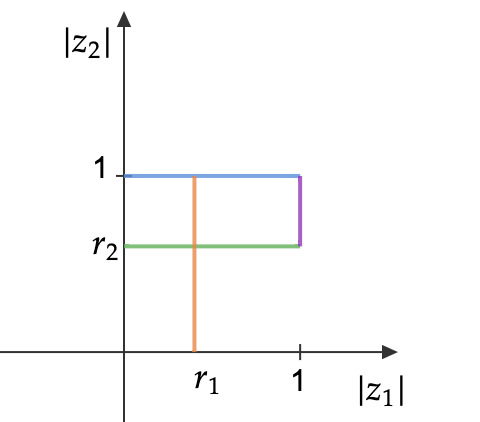
\includegraphics[width=0.4\textwidth]{Hartogs.jpg}
    \caption{Hartogs图}
    \end{figure}
  
  \begin{proof}
    令$r_2<r_3<1$, 对于$(z_1,z_2) \in \Delta \times \Delta _{r_3}$, 令
    $$ F(z_1,z_2)= \frac{1}{2\pi i} \int_{|\xi |=r_3}^{} \frac{f(z_1,\xi )}{\xi -z_2} d\xi,$$
    $\Rightarrow $ $F \in \mathcal{O}(\Delta \times \Delta _{r_3})$, 且 $F=f$ 于 $ \Delta_{r_1} \times \Delta _{r_3}$. 由唯一性定理 $\Rightarrow $ $F$ 为 $f$ 在 $ \Delta \times \Delta _{r_3}$上的全纯延拓.   
  \end{proof}
\end{example}

\begin{theorem}[Hartogs延拓定理]
    $\Omega $区域, $n \geq 2$. $K \subset \Omega $紧集且$\Omega \setminus K $连通.\\
    $\Rightarrow $ $\forall f \in \mathcal{O}(\Omega \setminus K)$可全纯延拓到$\Omega $.    
\end{theorem}
\begin{figure}[h!]
  \centering
  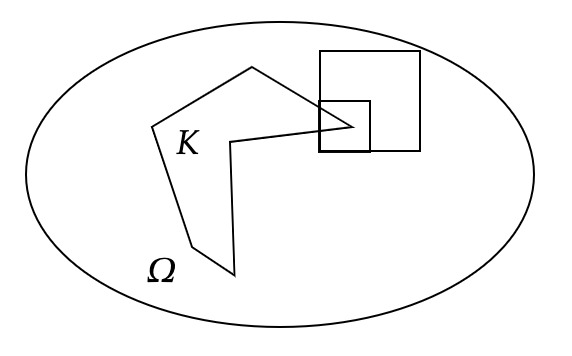
\includegraphics[width=0.4\textwidth]{Hartogs2.jpg}
  \caption{Hartogs的初等证明(Bochner给出完整的证明)}
  \end{figure}

\noindent\textbf{预备知识}:

\noindent 设$\Omega \subset \cc^n$为一区域, $v_1,...,v_n$为$\Omega $上$n$个函数. 称
$$ \frac{\partial u}{\partial \bar{z}_j}=v_j,\quad \forall  j=1,\dots,n  $$  
为非齐次Cauchy-Riemann方程.

令$v:=\sum_{j}^{}v_j d \bar{z}_j$ 为一 $(0,1)$-形式. 则 
$$ \bar{\partial}u=v, $$ 
$\because \quad \bar{\partial}^2u=0$, $\Rightarrow $  方程有解的必要条件为$ \bar{\partial}v=0. $

\begin{exercise}
$\bar{\partial}v=0 \iff \frac{\partial v_j}{\partial \bar{z}_k}=\frac{\partial v_k}{\partial \bar{z}_j}  $. 
\end{exercise}

\begin{lemma}[$\bar{\partial}$-Poincare引理 ]
  $n \geq 2 $, $v$: $\cc^n$中$C^{\infty }$-$(0,1)$形式且具有紧支集, $\bar{\partial}v=0$.\\
  $\Rightarrow $ $ \exists u \in C_{0}^{\infty }(\cc^n)$, s.t. $\bar{\partial}u=v$, 且 $u $ 在$\cc^n \setminus \supp(v)$   的无界连通分支上$\equiv 0 $.   
\end{lemma}

\begin{proof}[Hartogs延拓定理]
  取区域$\Omega ' \subset \subset \Omega , K \subset \Omega '.$ 取$\chi = C_0 ^{\infty }(\Omega ')$, $\chi \equiv 1$于$K $的某个领域. \\
  设$f \in \mathcal{O}(\Omega \setminus K)$. 令
  $$ v=\begin{cases}
     \bar{\partial}((1-\chi )f) &\text{} \Omega \setminus K\\
    0 &\text{} K \cup (\cc^n \setminus \Omega) \\
  \end{cases}  $$
  则$v$为 $\cc^n$中$C^{\infty }$-$(0,1)$形式且具有紧支集.\\
  $\Rightarrow \bar{\partial}u=v.$\\
  令 $F:=(1-\chi )f-u ~ \in C^{\infty }(\Omega )$, $\bar{\partial}F=v-\bar{\partial}u=0 \quad \Omega $. \\
  $\Rightarrow $  $F \in \mathcal{O}(\Omega )$.\\
  在 $\Omega \setminus \Omega ' $上, $u=0,\chi =0.$ (\textcolor{purple}{$ \bar{\partial }f=0 \Rightarrow \supp(v) \subset \supp (\chi ) \subset \Omega '$}. )    \\
  $\Rightarrow $ $F=f$于$\Omega \setminus \Omega '$.\\
  由唯一性定理, $\Rightarrow $ $F=f$ 于 $\Omega \setminus  K$.       
\end{proof}

\begin{lemma}\label{le:12}
设 $v=g d \bar{z}, g \in C_0^{\infty }(\cc)$. 令 $u(z)=\frac{1}{2 \pi i} \int_{\cc}^{} \frac{g(\xi )}{\xi -z} d \xi \wedge d \bar{\xi }.$ \\
则 $u \in C^{\infty }( \cc)$且 $\bar{\partial }u=v.$     
\end{lemma}
\begin{proof}
  令 $\xi =z+r e^{i \theta }$. \\
  $\Rightarrow $ $d \xi \wedge  d \bar{\xi }=-2ir dr \wedge  d \theta  $ $\quad (d \xi = e^{i \theta } dr +r i e^{i \theta } d \theta , d \bar \xi = e^{-i \theta } dr -r i e^{-i \theta } d \theta)$  \\
  $\Rightarrow $ $ u(z)=- \frac{1}{\pi }\int_{0}^{+\infty } \int_{0}^{2 \pi } g(z+r e ^{i \theta }) e^{-i \theta } dr d \theta $\\
  $\Rightarrow $ $ u \in  C^{\infty }(\cc)$\\
  $$  
  \begin{aligned}
    \Rightarrow \quad \frac{\partial u}{\partial \bar{z}}=&- \frac{1}{\pi } \int_{0}^{+ \infty } \int_{0}^{2 \pi } \frac{\partial g}{\partial \bar{z}} (z+r e^{i \theta })dr  d \theta    \\
    \stackrel{\xi =re^{i \theta }}{= } &  \frac{1}{2 \pi  i} \int_{\cc}^{} \frac{\partial g(z+\xi )}{\partial \bar{z}} \frac{1}{\xi }  d \xi \wedge d \bar{\xi } \\
    =& \frac{1}{2 \pi  i} \int_{\cc}^{} \frac{\partial g(z+\xi )}{\partial \bar{\xi }} \frac{1}{\xi }  d \xi \wedge d \bar{\xi } \\
    =& \lim_{\epsilon  \to 0}  \frac{1}{2 \pi i} \int_{\cc \setminus \bar{\Delta }_{\epsilon }}^{} \frac{\partial g(z+\xi )}{\partial \bar{\xi }} \frac{d \xi \wedge d \bar{\xi }}{\xi }  \\
    =& -\lim_{\epsilon  \to 0}  \frac{1}{2 \pi i} \int_{\cc \setminus \bar{\Delta }_{\epsilon }} d_{\xi } \left( \frac{g(z+\xi )}{\xi }d \xi \right)   \\
    \stackrel{Stokes}{= } & -\lim_{\epsilon  \to 0}  \frac{1}{2 \pi i} \int_{\partial  \bar{\Delta }_{\epsilon }}   \frac{g(z+\xi )}{\xi }d \xi   \quad (\textcolor{purple}{\text{令} \xi =\epsilon e^{i \theta }})\\
    =& g(z).
  \end{aligned} 
  $$      ~
\end{proof}

\begin{proof}[$\bar{\partial }$-Poincar\'e引理 ]
  设 $v:=\sum v_j d \bar z_j$. 则令 $z'=(z_2,\dots, z_n)$,
  $$ u(z):= \frac{1}{2 \pi i} \int_{\cc}^{} \frac{v_1(\xi ,z')}{\xi -z_1} d \xi  \wedge  d \bar{\xi }.$$  
利用极坐标 $\Rightarrow $ $u \in  C^{\infty }(\cc^n)$.\\
$ \text{由引理}\ref{le:12} \Rightarrow   $  $\frac{\partial u}{\partial \bar{z}_1} =v_1$.  \\
对于 $j \geq 2$,
$$ \begin{aligned}
  \frac{\partial u}{\partial \bar{z}_j}=& \frac{\partial }{\partial \bar{z}_j}  \left(\frac{1}{2 \pi i} \int_{\cc}^{} \frac{v_1(z_1+\xi ,z')}{\xi } d \xi  \wedge  d \bar{\xi }\right)\\
  =& \frac{1}{2 \pi i} \int_{\cc} \frac{\partial v_1}{\partial \bar{z}_j}(z_1+\xi ,z') \frac{d \xi  \wedge  d \bar{\xi }}{\xi } \\
  \stackrel{\text{由相容性条件}}{=}& \frac{1}{2 \pi i} \int_{\cc} \frac{\partial v_j}{\partial \bar{z}_1}(z_1+\xi ,z') \frac{d \xi  \wedge  d \bar{\xi }}{\xi } \\
  =& \frac{\partial }{\partial \bar{z}_1} \left(\frac{1}{2 \pi  i} \int_{\cc} \frac{v_j(z_1+\xi ,z')}{\xi }  d \xi  \wedge  d \bar{\xi }\right) \\
  \stackrel{\text{由引理}\ref{le:12}}{=}& v_j(z), \qquad \Rightarrow \bar{\partial }u=v.
\end{aligned} 
 $$ 
 $\because ~ v=0$ 于 $\cc^n \setminus \supp v$, $\Rightarrow  u \in \mathcal{O}(\cc^n \setminus \supp v)$.\\

 \begin{figure}[htbp]
  \centering
  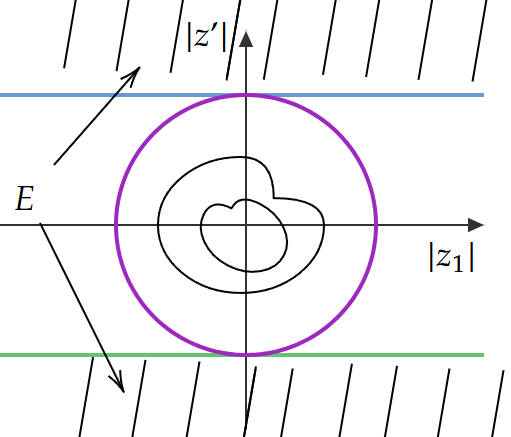
\includegraphics[width=0.4\textwidth]{DBarlem.jpg}
  \caption{$\db$-Poincare 引理证明}
\end{figure}
 取 $R>>1, \supp v \subset B(0,R)$, 则 $E=\{z \in \cc^n: |z'|>R \} \subset \cc^n \setminus B(0,R)$. 由 $u$的定义 $\Rightarrow $ $u|_E=0$ $ \overset{\text{唯一性}}{\Rightarrow}$ $u=0$ 于 $\cc^n \setminus \supp v $的无界连通分支.          
\end{proof}
 

\section{全纯映射}
$\Omega \subset \cc^n $ 区域, $F=(f_1,\dots,f_m)$为 $\Omega  \to \cc^n$的一个映射. 若 $\forall f_j \in \mathcal{O}(\Omega )$, 则$F$为一个全纯映射.
当$m=n$时, 则称
$$ J_{\cc}(F)=
\begin{vmatrix}
\frac{\partial f_1}{\partial z_1} & \cdots& \frac{\partial f_1}{\partial z_n}\\
\vdots & &  \vdots \\
\frac{\partial f_n}{\partial z_1} & \cdots& \frac{\partial f_n}{\partial z_n}\\
\end{vmatrix} $$
为$F$的复Jacobian. 

设 $ f_j=u_j+iu_{n+j}, j=1,\dots,n. \quad (z_j=x_j+ix_{n+j})$. 称 
$$ J_{\rr}(F)=
\begin{vmatrix}
\frac{\partial u_1}{\partial x_1} & \cdots& \frac{\partial u_1}{\partial x_{2n}}\\
\vdots & &  \vdots \\
\frac{\partial u_{2n}}{\partial x_1} & \cdots& \frac{\partial u_{2n}}{\partial x_{2n}}\\
\end{vmatrix} $$
为$F$的实Jacobian. 

\begin{proposition}\label{pro1}
$ J_{\rr} (F)=|J_{\cc}(F)|^2.$ 
\end{proposition}
\begin{corollary}
复流形可定向. 
\end{corollary}
\begin{proof}
  在 $ J_{\rr} $中第$n+r$行 $ \times i ~+$ 第$r$行, 利用 
  $$ \frac{\partial f_k}{\partial x_j} = \frac{\partial f_k}{\partial z_j} ,\quad \frac{\partial f_k}{\partial x_{n+j}}=i \frac{\partial f_k}{\partial z_j}   $$
  $$ \Rightarrow \quad  J_{\rr}=
  \left|
\begin{array}{c|c}
A & B \\
\hline
C & D
\end{array}
\right| $$
再将第$k$列 $ \times  -i$ $ + $ 第$n+k$列, 利用 
$$ \frac{\partial u_{n+j}}{\partial x_{n+k}} = \frac{\partial u_{j}}{\partial x_{k}}$$
$$ \Rightarrow \quad \left|
  \begin{array}{c|c}
  J_{\cc} & O \\
  \hline
  * & \bar{J}_{\cc}
  \end{array}
  \right| = \left| J_{\cc} \right|^2. $$ ~
\end{proof}

\begin{theorem}[隐函数定理]
 设 $ F(w,z)=(f_1(w,z),\dots,f_m(w,z)) $ 在 $ (0,0) $的某个领域内全纯, s.t. $ F(0,0)=0 $ 且 $ J_{\cc}(F)|_{(0,0)} \neq 0 $.\\
 $ \Rightarrow  $ $ \exists 0 \in \cc^n $ 的某领域上的全纯映射 $ w=w(z) $, s.t. $ w(0)=0 , F(w(z),z)=0$.
\end{theorem}
\begin{proof}
  令 $ w_k=u_k+iu_{n+k},z_k=x_k+i x_{n+k} $, 则 $ F(w,z)=0 $ 等价于下面 $ 2m $ 个实方程组
  $$\left\{  \begin{aligned}
    \Re F(u,x)=0 \\
   \Im F(u,x)=0 \\
  \end{aligned} \right. $$
  由命题 \ref{pro1} 及实隐函数定理 $ \Rightarrow  $ 
  $ \exists 0 \in \cc^n $的某个领域上的 $ C^{\infty } $ 映射 $ w $, s.t. 
  $$ w(0)=0, \quad F(w(z),z)=0. $$
  只需要证明 $ w $ 全纯:\\
  对方程 $ f_j(w(z),z)=0 $ 两边左边作用 $ \frac{\partial }{\partial \bar{z}_l}  $:
  $$ \sum_{k=1}^{m} \frac{\partial f_j}{\partial w_k} \frac{\partial w_k}{\partial \bar{z}_l} +\sum_{k=1}^{m} \frac{\partial f_j}{\partial \bar w_k} \frac{\partial \bar w_k}{\partial \bar{z}_l}=0$$
  $ \left(\left. \frac{\partial f_j}{\partial w_k}\right|_{(0,0)} \right)$为非异阵 $ \Rightarrow  $ $  \frac{\partial w_k}{\partial \bar{z}_l}=0 $于 $ 0 \in \cc^n $充分小的领域.
\end{proof}

\begin{corollary}[逆映射定理]
 $ U $ 为 $ w_0 \in \cc^n $ 的领域, $ G: U \to \cc^n $ 全纯. 且 $ z_0 =G(w_0), J_{\cc}(G)|_w \neq 0$. \\
 $ \Rightarrow  $ 在 $z_0 \in \cc^n$ 的某领域上$G^{-1}$ 存在且全纯.
\end{corollary}
\begin{proof}
  令 $ F(w,z)=G(w)-z $.
\end{proof}

\begin{corollary}
$ F:\Omega \subset \cc^n \to \cc^n  $全纯且 $ |J_{\cc}F|>0 $于 $ \Omega  $.\\
$ \Rightarrow  $ $ F $为一个开映射.
\end{corollary}
\begin{remark}
  \textcolor{blue}{单复变全纯 $ \Rightarrow  $ 开映射.}
\end{remark}

\begin{definition}
  $ F: \Omega  \subset \cc^n \to \Omega ' \subset \cc^n $ 为一个双射, 且$F^{-1} $ 全纯. 称 $F$ 为一个双全纯函数(Biholomorphic).

\noindent (\textcolor{blue}{由单复变启发, 对高维区域分类?})
\end{definition}
\begin{remark}
  $ \because F \circ F^{-1}=id $ $ \Rightarrow  $ $ J_{\cc} F \cdot J_{\cc}F^{-1}=1 $ $ \Rightarrow  $ $ |J_{\cc}F|>0 $. 反之, 若一个全纯映射$F $, s.t. $ |J_{\cc}F|>0 $, 则其局部为双全纯.
\end{remark}
\begin{example}[覆盖映射]
\begin{figure}[htbp]
  \centering
  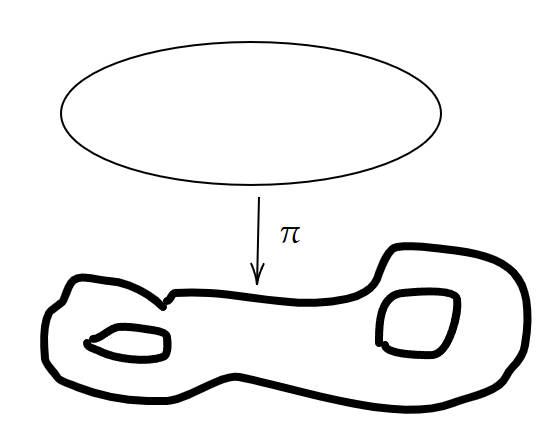
\includegraphics[width=0.4\textwidth]{Covering.jpg}
  \caption{覆盖映射}
\end{figure}  
\end{example}

\begin{theorem}[秩定理]
 $ \Omega \subset \cc^n $ 区域, $ 0 \in \Omega , F \in \mathcal{O}(\Omega ,\cc^m) $, s.t. $ F(0)=0 $
 且 $ F' $  的秩为常数 $ l. $
 则 $ \exists 0 \in \cc^n $ 以及 $ 0 \in \cc^m $ 领域上的双全纯映射 $ H,G $, s.t. $ G \circ F \circ H(w)=(w_1,\dots,w_l,0,\dots,0) $.
\end{theorem}
\begin{proof}
  设 $ F=(f_1,\dots,f_m) $
  不妨设 $ \det (\frac{\partial f_j}{\partial z_k} )_{1 \leq j,k \leq l}|_{0} \neq  0 $.
  定义全纯映射
  $$ A:\begin{cases}
   w_j=f_j(z)  &\text{} 1 \leq j \leq l\\
   w_j=z_j  &\text{} l+1 \leq j \leq n\\
  \end{cases}  $$
 $ \therefore $  $\exists 0 \in \cc^n $ 的某个领域上的 $ H=A^{-1} $.\\
$ \Rightarrow  $ $ A \circ H(w)=w $.\\
$ \Rightarrow  $ $ F \circ  H(w) = (w_1,\dots w_l, \tilde{f}_{l+1}(w),\dots, \tilde{f}_{m}(w))$ \\
 $ \because  $ $ F' $的秩为 $ l $, \\
 $ \Rightarrow  $ $ \frac{\partial \widetilde{f}_j}{\partial w_k} =0, \forall j,k >l $ 
 $$ \left|
  \begin{array}{c|c}
  J_{l \times  l} & O \\
  \hline
  * & \cdots 
  \end{array}
  \right|  $$
 $ \Rightarrow  $ $ \tilde{f}_j(w)= \tilde{f}_j(w_1,\dots, w_l) $.
 
 定义: $ G=(g_1,\dots,g_m) $
$$ \begin{cases}
  g_j(\xi )=\xi _j &\text{} j \leq l\\
  g_j(\xi )=\xi _j -\tilde{f}_j (\xi_1 ,\dots,\xi_l )&\text{} j>l\\
\end{cases}  $$
$ \Rightarrow  $ $ J_\cc(G)|_0 \neq 0 $ \\
$ \Rightarrow  $ $ G $ 在$0$ 的领域双全纯,
  且 $ G \circ F \circ H(w)=(w_1,\dots,w_l,0,\dots,0) $.
\end{proof}

\begin{lemma}[Schwarz引理]
 设 $ ||\cdot ||_1,||\cdot ||_2 $  为 $ \cc^n $ 中两个范数.
 $ B_1:=\{z \in \cc^n: ||z||_1 <1\} ,  B_2:=\{z \in \cc^n: ||z||_2 <1\}$
 若 $ F \in \mathcal{O}(B_1,B_2) $, s.t. $ F(0)=0 $.
 则 $ ||F(z)||_2 \leq ||z||_1 $.
\end{lemma}

\begin{example}
  $ ||z||_1 = \sqrt{|z_1|^2+\dots +|z_n|^2}$, 
  $ ||z||_2 =\max_{1 \leq j \leq n} |z_j| $.
\end{example}

\begin{theorem}[Poincare 定理]
 当 $ n \geq 2 $ 时, 单位球不双全纯同胚于单位多圆柱.
\end{theorem}
\begin{proof}
  $ F: \Delta^n \to  \mathbb{B}^n$. \\
  设 $ F(p)=0 $, 取 $ \phi _j \in \aut (\Delta ) $, s.t. $ \phi _j(p_j)=0 $. (\textcolor{blue}{单复变:$\aut (\Delta )=\{\text{莫比乌斯变换}\} $. $ \aut(\Omega )=\{f: \Omega \to \Omega \text{双全纯}\} $). }\\
  $ \Rightarrow  $ $ \phi := (\phi _1,\dots,\phi _n) \in \aut (\Delta ^n) $. \\
  令 $ G:=F \circ \phi ^{-1} $. 则 $ G $ 为双全纯且 $ G(0)=0 $. \\
  令 $ H=G^{-1} $, 对 $ G $ 以及$H$ 分别用 Schwarz引理 \\
  $ \Rightarrow  $ $ \sum |g_j(z)|^2=\max_{1\leq j \leq n}|z_j|^2  $.\\
  $ \because  $ 左边是 $ C^{\infty } $, 右边不是 $ C^{\infty } $. ($ \because  n \geq 2$.)
\end{proof}

\begin{lemma}[\textcolor{blue}{凸分析理论}]\label{le:14}
 设 $ ||\cdot|| $ 为 $ \cc^n $ 中的一个范数, $ z_0 \in \cc^n $.\\
 $ \Rightarrow  $ 存在一个复线性函数 $ l(z) $, s.t.
 $$ l(z_0)=||z_0||,\quad l(z) \leq ||z||, \forall  z. $$
\end{lemma}

\begin{proof}[Schwarz引理]
  $ \forall  z_0 \in B_1 \setminus \{0\} $, 由引理 \ref{le:14}, 存在复线性函数 $ l(w) $, s.t. 
  $$ l(F(z_0))=||F(z_0)||_2, \quad |l(w)| \leq ||w||_2, \forall w \in \cc^n. $$
  令 $ f(\xi ):=l \circ  F(\xi \frac{z_0}{||z_0||_1}), ~ \xi \in \Delta   $. \\
  对 $ f $ 用单复变 Schwarz引理,
  $$ |f(\xi )| \leq |\xi |, $$
  取 $ \xi =||z_0|| $ 代入.
\end{proof}

\begin{proof}[引理\ref{le:14}]
  令 $\Lambda  =\{(z,y)\in \cc^n \times \rr: y >||z|| \}$, 则 $\Lambda  $ 为凸集.(\textcolor{blue}{练习}) \\
  设 $(z_0,y_0) \in \partial \Lambda  $. 记 $E=\{\lambda \geq 0: \lambda \cdot (z_0,y_0)\} \subset \partial \Lambda  $.\\
  由 $\Lambda  $  凸性  $\Rightarrow $ 存在实超平面 $H$, s.t. 
  $$ E \subset H, H \cap \Lambda =\emptyset  \quad 0 \in H. $$ 
  $\Rightarrow $ $H=\{y=\Re l(z)\}$, $l$  为 $\cc^n $中的一个复线性函数.\\
  $\Rightarrow $ $y_0=\Re l(z_0)$. $(\because ~(z_0,y_0) \in H)$    \\
  $\Rightarrow $ $\Re l(z) \leq ||z||, \forall z \in \cc^n$.\\
  令 $\theta =\arg l(z)$, 则
  $\Rightarrow $ $\Re l(e^{-i \theta }z)~(=|l(z|)) \leq ||z||$. \\
  由 $\Re l(z_0)=||z_0||, |l(z_0)|=||z_0||$     $\Rightarrow $ $l(z_0)=||z_0||.$   
\end{proof}
\begin{remark}
   \textcolor{blue}{普林斯顿的分析教材: 实分析, 复分析, 傅里叶分析, 泛函分析, 还有凸分析. }
\end{remark}

\begin{theorem}[Cartan 唯一性定理]
    设 $\Omega \in \cc^n$  为一个有界区域, $F \in \mathcal{O}(\Omega ,\Omega )$. 
    若 $\exists P \in \Omega $ s.t. $F(p)=p, F'(p)=I$,   
    则 $F(z)=z, ~ \forall z \in \Omega $. 
\end{theorem}
\begin{proof}
  设 $ p=0, F=(f_1,\dots,f_n) $.
  幂级数展开: 
  $$ f_j(z)=z_j+\sum_{k=2}^{\infty }\underbrace{\sum_{|\alpha | =k} a_{\alpha }^{(j)}z^{\alpha } }_{p_k^{(j)}(z)}.$$
令 $ p_{k}(z)=(p_k^{(1)}(z),\dots,p_k^{(n)}(z)) $, 则 
$$ F=z+p_2(z)+p_3(z)+\cdots . $$
$ \Omega  $ 有界, $ \Rightarrow  $ $ |F| \leq M $. 假设 $ F(z) \not \equiv z $, 则存在 $ m \leq 2 $, s.t. $ p_m(z)=0 $, 且 
$$ F(z)=z+p_m(z)+p_{m+1}(z)+\cdots.  $$
考虑 $ F $的$k$次迭代, $ F^k=F \circ \cdots \circ  F $. (\textcolor{blue}{动力系统框架之内.})
$$ \begin{aligned}
  F^2(z)=&z+p_m(z)+\cdots \\
  &+p_m(z+p_m(z)+\cdots)+\cdots \\
  =&z+2p_m(z)+\text{高阶项}(>2)
\end{aligned}  $$
$$
  F^k=z+kp_m(z)+\text{高阶项}.
$$
取多圆柱 $ P(0,r) \subset \subset \Omega , r <<1 $. 
由Cauchy不等式, $ \forall |\alpha| =m $, 
$$ k \left| a_{\alpha }^{(j)} \right|  \leq \frac{\alpha !}{r^{\alpha }}M .$$
令 $ k \to \infty  $, $ \Rightarrow  $ $  a_{\alpha }^{(j)}=0 $ $ \Rightarrow  $ $ p_m(z)\equiv  0 $, 矛盾.
\end{proof}

\begin{corollary}[Cartan]
 $ \Omega _1, \Omega _2 \subset \cc^n $ 中完备有界圆域. $ F \in \mathcal{O}(\Omega _1,\Omega _2) $ 双全纯 且 $ F(0)=0 $. 则 $ F $ 必为一个复线性映射, 即若 $ F=(f_1,\dots,f_n) $, 则 $ f_j(z)=\sum_{k=1}^{n} c_{jk}z_k $, $ c_{jk} \in \cc $.
 ($ F(z)=Az, A:=(c_{jk}) $.)
\end{corollary}
\begin{proof}
  对于 $\theta \in \rr$, 定义 
  $$ e^{i \theta }: z \mapsto e^{i \theta }z. $$ 
  记 $e^{-i \theta }$ 为 $e^{i \theta }$的逆. 令 $G=F^{-1}$, 则
  $$ H(z):= e^{-i \theta } G(e^{i \theta }F(z)) \in \mathcal{O}(\Omega _1, \Omega _2),$$   
  且 $H(0)=0,H'(0)=I$. 
  由唯一性, $\Rightarrow H(z)=z$.\\
  $\Rightarrow  e^{i \theta }F(z)=F(z e ^{i \theta })$, $\Leftrightarrow e^{i \theta }f_j(z)=f_j(z e^{i \theta })$.\\
  两边作用 $\partial ^\alpha =\frac{\partial^{|\alpha |} }{\partial z^{\alpha }}$,    再取 $z=0$: 
  $$ e^{i \theta } \partial ^{\alpha } f_j(0)=e^{i |\alpha | \theta } \partial ^{\alpha } f_j(0), \quad \forall \theta \in \rr.$$       
  $\Rightarrow $ 当 $|\alpha| \geq 2$  时, $\partial ^{\alpha }f_j(0)=0$.\\
  $\Rightarrow F$ 为线性函数.     
\end{proof}

\begin{theorem}
  $\forall F \in \aut(\Delta ^n)$ 必可写成 \\
   $$ \left( e^{i \theta _1} \frac{z_1-p_1}{1-\bar p_1 z_1},\ldots , e^{i \theta _n} \frac{z_n-p_n}{1-\bar p_n z_n}\right), \quad (1)$$ 
   (某个 $ p=(p_1,\dots, p_n) \in \Delta ^n, \theta _1,\dots,\theta _n \in \rr$) 与某个置换的复合.  
\end{theorem}
\begin{proof}
  设 $F(p)=0$. 
  取
  $$ G(z)=\left( \frac{z_1-p_1}{1-\bar p_1 z_1},\ldots ,  \frac{z_n-p_n}{1-\bar p_n z_n}\right) \in \aut (\Delta ^n), $$
  且 $s.t. G(p)=0$. \\
  $\Rightarrow G \circ F^{-1} \in \aut (\Delta ^n), ~ 0 \mapsto 0.$\\
  $\Rightarrow G \circ F^{-1}$ 为线性映射, 即若 $G \circ F^{-1}=(g_1,\dots,g_n)$  
  则  $g_j(w)=\sum_{k=1}^{n}c_{jk}w_k$. \\
  对 $r<1$, 
  取 $w_k=r e^{-i \arg (c_{jk})}$ 代入 \\
  $\Rightarrow 1 > |g_j(w)|=r \sum_{k=1}^{n}|c_{jk}|$. \\
  令 $r \to 1$ 
  得 
  $$ \sum_{k=1}^{n}\left| c_{jk} \right| \leq 1, \quad 1 \leq j \leq n.  \quad (*) $$

  由 Schwarz 引理 (\textcolor{purple}{对 $G \circ F^{-1}$  和 $(G \circ F^{-1})^{-1}$ 应用})
  $$ \max \{ |\sum_{k}^{} c_{1k}w_k|,\dots, |\sum_{k}^{} c_{nk}w_k|\} =\max \left\{ |w_1|,\dots,|w_n| \right\}. $$
  对固定 $k$, 
  令 $w_k=r, 0 < r<1, w_l=0, l \neq k$ 
  代入, 
  再令 $r \to 1$: 
  $$  \max \{ | c_{1k}|,\dots, | c_{nk}|\}=1\quad (**) $$ 
  令
  $$ A=\begin{pmatrix}
c_{11} & \cdots  & c_{1n} \\
c_{21} & \cdots  & c_{2n} \\
\vdots  &  \ddots  & \vdots  \\
c_{n1} & \cdots  & c_{nn}
\end{pmatrix} ,$$
$(*),(**)$ $\Rightarrow $ $A$ 的每一行每一列只有一个非零元, 且 模 为 $1$. \\
$\Rightarrow F $ 为 $(1)$ 与某个置换的复合.     
\end{proof}

\begin{lemma}
  设 $F \in \aut(\mathbb{B}^n)$ 
  且 $F(0)=0$. 
  则 $F$  为酉变换, 即 $F(z)=z \cdot U$, $U$ 为酉阵.  
\end{lemma}
\begin{proof}
  由之前的推论, $F$ 为线性的, $F(z)=z \cdot U$, $U$ 为非异阵. \\
  设 $z \in \mathbb{B}^n \setminus \{0\}$, 
  目标: $|z|=|z \cdot U|$ ($\Rightarrow U$ 为酉阵). \\
  假设 $|z| < |z U|$.
  $\Rightarrow \frac{z}{|zU|} \in \mathbb{B}^n,$ $\Rightarrow F(\frac{z}{|zU|})=\frac{zU}{|zU|} \in \partial \mathbb{B}^n$, 矛盾.\\
  若 $|z| \geq |zU|$, $\frac{zU}{|z|} \in \mathbb{B}^n$, $\Rightarrow F^{-1}\left(\frac{zU}{|z|}\right)\in \partial \mathbb{B}^n$, 矛盾.      
\end{proof}


设 $z'=(z_2,\dots,z_n)$. 
设 $a \in \Delta $. 希望找到 $\Phi _a \in \aut (\mathbb{B}^n)$, s.t. $\Phi _a(a,0')=0.$   \\
取 $w_1 = \frac{z_1-a}{1-\bar a z_1}$. 利用 ($\because z \in \mathbb{B}^n $  )
$$ 1-|w_1|^2=1-\frac{|z_1-a|^2}{|1-\bar a z_1|^2} =\frac{(1-|a|^2)(1-|z_1|^2)}{|1-\bar a z_1|^2} > \frac{(1-|a|^2)}{|1-\bar a z_1|^2}|z'|^2,  $$
令 $w'=\frac{\sqrt{1-|a|^2}}{1-\bar a z_1} z'$. 
作 $\Phi _a(z)= \left( \frac{z_1-a}{1-\bar a z_1},\frac{\sqrt{1-|a|^2}}{1-\bar a z_1} z' \right) \in \mathcal{O}(\mathbb{B}^n, \mathbb{B}^n)$, s.t. $ \Phi _a(a,0')=0$.\\
类似, 令 $\Psi _a(w)=\left( \frac{w_1+a}{1+\bar a w_1},\frac{\sqrt{1-|a|^2}}{1-\bar a w_1} w'\right) \in  \mathcal{O}(\mathbb{B}^n, \mathbb{B}^n)$. 则 $\Psi_a \circ \Phi _a =\id$.     

\begin{theorem}
  $\forall F \in \aut(\mathbb{B}^n)$ 可以写成 
  $$ F=U_1 \circ \Phi _{|F(0)|}^{-1} \circ U_2 ,$$ 
  $U_1,U_2$ 为酉变换.  
\end{theorem}
\begin{proof}
  取酉变换 $U_1$, s.t. $U_1^{-1} \circ F(0)=(|F(0)|,0')$.  \\
  $\because~ \Phi _{|F(0)|}\circ U_{1}^{-1} \circ F \in \aut (\mathbb{B}^n)  $, s.t. $0 \mapsto 0$. 
  由引理 $\Rightarrow \Phi _{|F(0)|}\circ U_{1}^{-1} \circ F=U_2$, $U_2$ 为酉阵.     
\end{proof}

\noindent\textbf{Corona(日冕问题)} 设 $f_1,\dots,f_m$ 为 $\mathbb{B}^n$ 或 $\Delta ^n (n \geq 2)$   上有界全纯函数. 且 $\exists \delta >0,$ s.t. $\sum_{i=1}^{m}|f_i| \geq \delta $. 问题: 是否存在有界全纯函数 $g_1,\dots,g_m$, s.t. $\sum_{j=1}^{m}f_jg_j=1$?    

\begin{itemize}
\item 单位圆盘的情形由 L. Carlson 解决.
\item Varopolous 解决了BMO空间的情形.
\end{itemize}

\begin{definition}
  设 $\Omega  \subset \cc^n$ 为一个有界区域, 若 $\forall a,b \in \Omega $, $\exists F \in \aut(\Omega )$, s.t. $F(a)=b$, 则称 $\Omega $ 为一个齐性域. 进一步, 若 $F(b)=a$, 则称 $\Omega $ 为一个对称域.       
\end{definition}

\begin{example}
  $\Delta ^n, \mathbb{B}^n$ 均为对称域. 
\end{example}

\begin{remark}
  $\aut(\cc)=\{az+b|a \neq 0\}$. 当 $n \geq 2$时, $\aut(\cc^n)$ 远远来的复杂.   
\end{remark}
\begin{example}
  设 $f \in \mathcal{O}(\cc)$. 定义
  $$ \begin{aligned}
    F: &\cc^2 \to \cc^2\\
    & (z_1,z_2) \mapsto (z_1,z_2+f(z_1)).
  \end{aligned} 
   $$ 
则 $F^{-1}(w_1,w_2)=(w_1,w_2-f(w_1))$, $\Rightarrow F \in \aut (\cc^2)$.  
\end{example}


\begin{theorem}\label{thm3}
  $F=(f_1,f_2)$, $f_1,f_2$ 为 $\cc^2$ 中二阶多项式. 若 $\underline{F(0)=0, F'(0)=I}$ \textcolor{red}{(可去掉)}. 
  且 $\det F'(z) \equiv 1$, 则 $F \in \aut (\cc^2)$.      
\end{theorem}
\begin{proof}
  设 $f_j=z_j+a_j z_{1}^{2}+b_j z_1 z_2+c_j z_{2}^{2}, ~j=1,2$.
  $$ \det F'=1 \Leftrightarrow \begin{cases}
    2 a_1z_1+b_1z_{2}+b_2 z_1+2c_2z_2=0, &\text{}\\
    \begin{vmatrix}
      2a_1z_1+b_1z_2 & b_1z_1+2c_1z_2\\
      2a_2z_1+b_2z_2 & b_2z_1+2c_2z_2
    \end{vmatrix}=0.
     &\text{}
  \end{cases} \quad (\text{\textcolor{red}{练习}})$$
$\Rightarrow \frac{a_2}{a_1}=\frac{b_2}{b_1}=\frac{c_2}{c_1}:=d$,  
$b_1=- \frac{2a_1}{d},c_1=\frac{a_1}{d^2}$. \\
$$\Rightarrow \quad \begin{cases}
  f_1=z_1+a_1(z_1-\frac{z_2}{d})^2 &\text{}\\
  f_2 =z_2+a_1 d(z_1-\frac{z_2}{d})^2.&\text{}
\end{cases} $$ 
令 $\xi =z_1-\frac{z_2}{d}$, 

$$ \Rightarrow ~ \begin{pmatrix}
  f_1\\
  f_2
\end{pmatrix}
= \begin{pmatrix}
  1 & 0\\
  d & 1
\end{pmatrix}
\begin{pmatrix}
  z_1+a_1 \xi ^2\\
  -d \xi 
\end{pmatrix}
\in \aut (\cc^2).
 $$
\end{proof}

\textbf{Jacobi 猜想}: 设 $F:\cc^n \to \cc^n $ 为一个多项式映射, s.t. $\det F' \equiv const.$. 则 $F \in \aut(\cc^n)$.   

\begin{remark}[Picard 小定理]
  若 $f \in \mathcal{O}(\cc), f \neq const.$,  
  则 $\#\{\cc \setminus f(\cc)\}\leq 1$. 
\end{remark}

\begin{theorem}
  存在 双全纯映射 $F:\cc^2 \to F(\cc^2) \subset \cc^2$, s.t. $\cc^2 \setminus F(\cc^2)$ 有内点.  
\end{theorem}
\begin{proof}
  构造概要(\textcolor{red}{复动力系统}).

  1. 令 
  $$ P:\begin{pmatrix}
    z_1 \\
    z_2
  \end{pmatrix}
  \mapsto 
  \begin{pmatrix}
    z_2 \\
    a^2z_1+(1-a^2)z_2^2
  \end{pmatrix}.
   $$
   $\Rightarrow \quad P'(z)=-a^2$, \\
   $\Rightarrow  \quad P \in \aut(\cc^2)$. (定理 \ref{thm3})\\
   记 $S:=\{z \in \cc^2: \lim_{k \to \infty }P^k(z) =0\}$.\\
   设 $0 <t \leq 1$, $\textcolor{purple}{(0<a<1)}$, 
   $$b_t=\frac{t+a^2}{t(1-a^2)}, \quad E_t=\left\{z \in \cc^2: \left|   \frac{z_2}{z_1}\right|\geq t,|z_2| \geq b_t\right\}.$$      
   $E_t \subset \cc^2 \setminus  S$: 
   $$ P=(p_1,p_2),z \in E_t \Rightarrow \left| \frac{p_2(z)}{p_1(z)} \right| \geq 1, \text{ 且 } \left| p_2(z) \right| \geq |z_2| \geq b_t  $$ 
   $\Rightarrow p^k(z)\in E_t$. $\because~ 0 \not\in E_t \Rightarrow z \not\in S $. 

2. 令 
$$ A: \begin{pmatrix}
    z_1 \\
    z_2
  \end{pmatrix}
  \mapsto 
  \begin{pmatrix}
    -a z_1 \\
    az_2
  \end{pmatrix} ,$$   
则 $\det A'=-a^2$. 
若 $\exists F \in \mathcal{O}(\cc^2,\cc^2)$, s.t. $F(0)=0, \det F'(0) \neq 0 $ 且 
$$ P \circ F = F \circ A, \quad (*)$$   
则 $F:\cc^2 \to S$ 为双全纯. \\
由 $(*)$ $\Rightarrow $ $ \textcolor{purple}{(\because ~ \det F'|_{Az} a^2=a^2 \det F'|_z )}$
$$ \det F' =\det F'\circ A = \cdots =\det F'\circ A^k ,$$
$\because ~ A^k \to 0 \Rightarrow \det F'=\det F'(0) \neq 0.$   \\
另一方面, $(*)\Rightarrow P^k \circ F=F \circ A^k$, i.e., $F=P^{-k}\circ F \circ A^{k}, ~ \forall k$, \\
$\Rightarrow F$ 局部双全纯, 且 $F$ 为单射.    

下证 $F(\cc^2)=S$: \\
$"\subset "$: $z=F(z') \Rightarrow P^k(z)=P^k \circ F(z')=F(A^k z') \to F(0)=0 ~(k \to \infty  ).$  \\
$"\supset "$: $z \in S \Rightarrow P^k(z) \to 0.$ 
$\because ~ F$ 在 $0$  附近双全纯, $F(\cc^2)$ 包含 $0$  的一个领域. \\
$\Rightarrow F(z')=P^k(z), ~ k \gg 1$, 
$\Rightarrow z=P^{-k}F(z')=F(A^{-k} z')$
$\Rightarrow z \in F(\cc^2)$.    

3. $(*)$ 的可解性, Ref: \textcolor{blue}{沙巴特:复分析导论II}. 
\end{proof}

\section{零点和极点}

单复变全纯函数: 零点是孤立的.

多复变($n \geq 2$): 零点不孤立. 根据 Hartogs 延拓定理, 设 $f \in \mathcal{O} ( \mathbb{B}^n), f(0)=0$. 若零点 $0$  是孤立的, 则 $\frac{1}{f} \in \mathcal{O} ( \mathbb{B}^n)$.  

\begin{theorem}[Riemann 可去奇性定理]
  $\Omega \subset \cc^n$ 区域, $0 \not \equiv g \in \mathcal{O}(\Omega ), A =g^{-1}(0)=\{z \in  \Omega :g(z)=0\}$. 
  若 $f \in \mathcal{O}(\Omega \setminus A)$ 
  且存在 $A$  的每一点附近有界, 则 $\exists ! \tilde{f} \in \mathcal{O}(\Omega )$, s.t. $\tilde{f}|_{\Omega \setminus A}=f$.    
\end{theorem}

\begin{proof}
  1. 只要证 $f$  可延拓为任一 $a \in A$  的一个领域上的全纯函数.

  2. 不妨设 $a=0$, 且 $g(0',z_n) \not \equiv 0, z'=(z_1,\dots,z_{n-1})$. (若$g(0)=0$, 可以考虑旋转平移. (\textcolor{red}{练习}) )  

  由单复变零点的孤立性, $\exists 0< \delta \ll 1$, s.t. $|g(0',z_n)|>0$ 于 $\partial \Delta (0, \delta )$. 
  由连续性, $\exists 0< \delta ' \ll 1$, s.t. $|g(z',z_n) |>0$ 于 $\Delta ^{n-1}(0,\delta ) \times \partial \Delta (0,\delta )$. \\
  $\Rightarrow \Delta ^{n-1}(0,\delta ) \times \partial \Delta (0,\delta ) \subset \Omega \setminus A$.
  
  3. 定义 
  $$ h(z',z_n)=\frac{1}{2 \pi  i} \int_{|\xi |=\delta } \frac{f(z',\xi )}{\xi -z_n} d \xi .$$
  $h$ 关于 $z' \in \Delta ^{n-1}(0,\delta '),z_n \in \Delta (0,\delta )$ 均全纯且局部有界, \\
   $\Rightarrow  h \in \mathcal{O}(\Delta ^{n-1}(0,\delta ') \times \Delta (0,\delta ))$.  \\
   任意固定 $z' \in \Delta ^{n-1}(0,\delta ')$. $\because ~ g(z',z_n)$ 在 $\{z'\} \times \Delta (0,\delta )$ 的零点是孤立的, $\therefore $ 由单复变 Riemann 可去奇性定理(\textcolor{red}{$f$ 在 $A$ 有界, 且只有有限个零点}), $f(z', \cdot )$ 可延拓 为 $\{z'\} \times \Delta (0.\delta )$ 上的全纯函数 $\tilde{f}(z',\cdot )$. 
   $$\begin{aligned}
    \because \quad \tilde{f}(z',z_n )=&\frac{1}{2 \pi  i} \int_{|\xi |=\delta } \frac{\tilde{f}(z',\xi )}{\xi -z_n} d \xi \\
    =&\frac{1}{2 \pi  i} \int_{|\xi |=\delta } \frac{f(z',\xi )}{\xi -z_n} d \xi \\
    =& h(z',z_n),
   \end{aligned}  $$      
   $\Rightarrow  \tilde{f} \in \mathcal{O}(\Delta ^{n-1}(0,\delta ') \times \Delta (0,\delta ))$ 为 $f$ 的全纯延拓. 
   
   唯一性由全纯函数的唯一性定理得.
\end{proof}

\begin{corollary}
  设 $\Omega \subset \cc^n,n \geq 2$  区域, $f,g \in \mathcal{O}(\Omega )$. 
  若存在紧集 $K \subset \Omega $, s.t. $\Omega \setminus K$ 连通 且 $|f| \leq |g|$ 于 $\Omega \setminus K$, 
  则 $|f| \leq |g|$ 于 $\Omega $.      
\end{corollary}
\begin{proof}
  令 $h=f/g$, $h \in \mathcal{O}(\Omega \setminus K \setminus g^{-1}(0))$. \\ 
  因为 $|h| \leq 1$  于 $\Omega \setminus K$, 由 Riemann 可去奇性定理 
  $\Rightarrow h \in \mathcal{O}(\Omega \setminus K)$.\\
  由 Hartogs延拓定理 $\Rightarrow h \in \mathcal{O}(\Omega )$, \\
  由最大模定理 $\Rightarrow |h| \leq 1$ 于 $\Omega $.   
\end{proof}

\begin{remark}
  $n=1$ 时 fail:
   $\Omega =\Delta ,f \equiv \frac{1}{2},g(z)=z$. 则 $|f| \leq |g|$ 于 $\Delta \setminus \bar{\Delta }_{\frac{1}{2}}$, 但 $|f(0)|=\frac{1}{2}>0=g(0)$.     
\end{remark}



\begin{definition}
  设 $\Omega \subset \cc^n$ 区域, $A \subset \Omega $. 若 $a \in \Omega $,  存在 $a$  的领域 $U \subset \Omega $ 以及 $f_1,\dots,f_k \in \mathcal{O}(U)$, s.t. $A \cap U=\cap _{j=1}^{k} f_{j}^{-1}(0)$, 则称 $A$  为 $\Omega $ 的一个{\sffamily\small 解析子集} (Analytic subset). 
  $k=1$ 时, 称 $A$ 为解析超平面.         
\end{definition}
\begin{remark}
  总假设 $A \subsetneq  \Omega $. 
\end{remark}

基本性质: \\
1. $A \subset \Omega $ 闭集(相对):
\begin{proof}
  设 $z_i \to z_0 \in \Omega, \{z_i\} \subset A $.  取 $z_0 \in U \subset \Omega $, 以及 $f_1,\dots,f_k \in \mathcal{O}(U)$, s.t. $\cap_{j=1}^{k} f_{j}^{-1}(0)=A \cap U$.  
  当 $m \gg 1$ 时, $z_m \in U$, $\Rightarrow f_j(0)=0, \forall j$.
  由连续性, $\Rightarrow f_j(z_0)=0, \forall j$. $\Rightarrow z_0 \in A$.     
\end{proof}
 2. 解析子集的有限交为解析子集.\\
 3. $\Omega \setminus A$ 连通: 
 \begin{proof}
  由于解析子集局部包含于一个解析超平面中, 所以只要证: 对任意 的 多圆柱 $P \subset \Omega $, 若 $A \cap P=g^{-1}(0), g \in \mathcal{O}(P)$, 则 $P \setminus A$ 连通.  \\
  取 $z,w \in P \setminus A$, 记 $H$ 为 $z,w$ 决定的复线($\cong \rr^2$), 即 其由 $\xi =tz+(1-t)w,t \in \cc$ 给出. $g|_{H \cap P}$ 关于 $t$ 全纯, 且 不恒为零($H \cap P$ 为平面). 由零点孤立性$\Rightarrow $ $A \cap H$ 离散 $\Rightarrow $ 存在折线 $\gamma \subset (H \setminus A) \cap P$ 连接 $z,w$. $\Rightarrow $ $P \setminus A$ 连通.             
 \end{proof}
4. $A$ 无内点($\Rightarrow \Omega \setminus A$ 在 $\Omega $ 中稠密). \textcolor{red}{$A$ is ``thin", not ``fat".  } 
\begin{proof}
  假设 $A^{\circ } \neq \emptyset  $. 
  设 $a \in \partial A^{\circ } \cap \Omega $.\\
   $\exists a \in U \subset \Omega , f_1,\dots,f_k \in \mathcal{O}(U)$, s.t. $\cap_{j} f_{j}^{-1}(0)=A \cap U$. \\
  所以 $f_j |_{U \cap A^{\circ }}=0, \forall j$
   $\Rightarrow $ $f_j=0$ 于 $U$   
   $\Rightarrow $ $U \subset A^{\circ }$ $\Rightarrow $ $A^{\circ }$ 闭 $\Rightarrow $ $A^{\circ }=\emptyset $. ($A^{\circ }=\Omega $不可能, 因为约定了 $A \neq \Omega $  ).       
\end{proof}

\begin{definition}
  设 $A \subsetneq \Omega $  为解析子集, $a \in A$, 若存在邻域 $ \Omega \supset U \ni a $  以及 $f_1,\dots,k_k \in \mathcal{O}(U)$, s.t. $A \cap U=\cap f_{j}^{-1}(0)$, 且全纯映射 $F=(f_1,\dots,f_k) \in \mathcal{O}(U,\cc^k)$ 满足 $\rank F'(a)=k$, 则称 $a$ 为 $A$ 的一个{\sffamily\small 光滑点(正则点)}.    
  若 $A$ 的每点都是光滑点, 则称 $A$ 为 $\Omega $ 的一个{\sffamily\small 复子流形}.  
  令
  $$ R(A):=\{a \in A: a \text{为光滑点}\} ,$$   
  则 $R(A) \subset A$ 为开集. 
\end{definition}
\begin{definition}
  称 $S(A):=A \setminus R(A)$ 为 $A$  的{\sffamily\small 奇点集} ($S(A) \subset A$ 为闭集). 
\end{definition}

\begin{example}
  令 $f(z_1,z_2)=z_1 z_2$, $A=f^{-1}(0)$ .
  则  $S(A)=\{(z_1,z_2)\in \cc^2| z_1=z_2=0\}$.  
\end{example}

\begin{definition}[维数]
  设 $A \subsetneq \Omega $ 为解析子集, $a \in A$. 若 $a \in R(A)$, 定义 $\dim_aA$ 为复子流形 $A \subset U$ 的维数, $U \ni a$ 为充分小邻域. 若 $a \in S(A)$, 定义 
  $$ \dim_aA:= \limsup_{R(A) \ni z \to a} \dim_zA .$$   
  定义 $A$ 的维数: 
  $$ \dim A:= \limsup _{a \in A} \dim_aA ,$$  
  称 $\codim A:=n-\dim A$ 为 $A$ 的余维数.     
\end{definition}

\begin{theorem}[解析子集的层化]
  存在解析子集 $A_1 \subset A$, s.t. $\dim A_1 <\dim A$ 且 $S(A) \subset A_1$ (局部也成立, 即 $\forall U$, $\dim A_1 \subset U <\dim A \subset U$  ).
  存在解析子集 $A_2 \subset A_1,\dim A_2 < \dim A_1,\dots,$ 经过有限步结束. 
  $$ \implies A= R(A) \cup R(A_1) \cup R(A_2) \cup \dots \cup \text{离散点列}, $$    
  称其为解析子集的层化.
\end{theorem}
\begin{remark}
  可以证明 $S(A) \subset A$ 为解析子集, 且 $\dim S(A) < \dim A$.  
\end{remark}
\begin{proof}
  设 $a \in S(A)$. 设 $k$ 为满足下列条件的最大整数: 存在邻域 $\Omega \supset U \ni a$  以及 $f_1,\dots,f_k \in \mathcal{O}(U)$ 满足\\
   (1) $A \cap U \subset  \cap _{j=1}^{k} f_{j}^{-1}(0)$; \\
   (2) $\big(\frac{\partial f_j}{\partial z_l}\big)$ 中有一个 $k$-阶子式 $D$ 在 $A \cap U$ 上不恒等于0.      \\
   目标: 证明 
   $$ S(A) \cap U \subset \{z \in A \cap U:D(z)=0\} .$$
   取 $V:=\{z \in U: D(z) \neq 0\}$, $\tilde{A}:=\cap _{j=1}^{k} f_{j}^{-1}(0) \cap V$. 则 $\tilde{A}$ 为一个复子流形 ($n-k$-维 ). 设 $z^0 \in \tilde{A}$. 不妨设 $D(z)=\det \big(\frac{\partial f_j}{\partial z_l}\big)_{j,l=1}^{k}$. 作坐标变换(秩定理)
   $$ \begin{cases}
    w_j=f_j(z) &\text{} j \leq k,\\
    w+j=z_j-z_{j}^{0} &\text{} j>k,\\
   \end{cases}  $$  
   $$\implies  \tilde{A} \cap U_0=\{w \in U_0: w_1=\dots=w_k=0\}$$    
   略.
\end{proof}

\begin{theorem}[Riemann可去奇性定理II]
  设$A \subset \Omega $ 为解析子集, s.t. $\codim A \geq 2$. 则 $\forall f \in \mathcal{O}(\Omega  \setminus A)$, $\exists ! \tilde{f} \in \mathcal{O}(\Omega )$, s.t. $\tilde{f}|_{\Omega \setminus A}=f$.     
\end{theorem}
\begin{proof}
  对 $k=\dim A$ 用归纳法. 
  当 $k=0$ 时, $A$ 为离散点列, 且 $\dim \Omega \geq 2$, 由 Hartogs延拓定理即得. 假设结论对 $k \leq m-1$ 时成立. 
  由 $A$ 的层化分解, 只要证 $f$ 可全纯延拓过 $\forall a \in R(A)$. 取复坐标 $z$ 以及多圆柱 $P=\Delta ^n(0,r)$, s.t. 
  $$ P \cap A =\{z \in P: z_1=\dots=z_{n-m}=0\} \subset \{z \in P: z_1=z_2=0\}. $$   
  令 $z'=(z_3,\dots,z_n)$, $\forall  z' \in \Delta ^{n-2}(0,r), f(\cdot ,z') \in \mathcal{O}(\Delta ^{2}(0,r)\setminus 0).$ 由 Hartogs延拓定理 $\implies f(\cdot ,z') \in \mathcal{O}(\Delta ^{2}(0,r))$. 由最大模定理 $$\implies |f(z)| \leq \max_{\partial \Delta ^{2}(0,r) \times \Delta ^{n-2}(0,r)}|f|.$$           
  所以 $f \in L^{\infty }(\Delta ^{n}(0,r))$, 由 Riemann可去奇性定理I 即得. 
\end{proof}

\begin{theorem}[$L^2$-Riemann可去奇性定理* ]
  设 $A \subset \Omega $ 为解析超曲面 
  则 
  $$ \mathcal{O}(\Omega \setminus A) \cap L^2_{loc}(\Omega )=\mathcal{O}(\Omega ) .$$
\end{theorem}
\begin{exercise}
  $L^p$ 的情形? 
\end{exercise}


\begin{definition}
  记 $\mathcal{O}_0$ 为 $0 \in \cc^n$ 的某邻域上的全纯函数全体. 记 $z'=(z_1,\dots,z_{n-1})$.  
\end{definition}

\begin{definition}
  设 $f \in \mathcal{O}_0, f(0)=0$. 若 $f(0',z_n) \not \equiv 0$, 则由单复变理论可知 $f(0',z_n)=z_n^k \phi (z_n), $ $\phi $ 全纯且 $\phi (0) \neq 0$. 此时称 $f$ 关于 $z_n$ 在原点 {\sffamily\small $k$ 阶正则}.    若 $P \in \mathcal{O}_0$ 可以写为 
  $$ P(z',z_n)=z_{n}^{k}+a_{k-1}(z')z_{n}^{k-1}+ \cdots +a_1(z')z_n+a_0(z') ,$$   
  其中 $a_j \in \mathcal{O}_{0'},a_j(0')=0$, 则称 $P$ 为 {\sffamily\small Weierstrass多项式(W-多项式)}.  
\end{definition}

\begin{theorem}[Weierstrass预备定理]
 设 $f$ 关于 $z_n$ 在原点 $k$ 阶正则, 那么存在原点某邻域上的 W-多项式 $P$ 以及全纯函数 $h$ s.t. 
  $$ f=Ph \quad \text{且 } \quad h(0) \neq 0.$$     
\end{theorem}
\begin{proof}
  存在 $0< \delta <<1$, s.t. $f(0',z_n)$ 在 $\overline{\Delta (0,\delta )}$  只有 $0$ 为零点.
  存在 $0<\delta ' <<1$, s.t. 
  $$ | f(z',z_n)-f(0,z_n) | < \min_{\partial \Delta (0,\delta )}|f(0',z_n)|, \quad \forall z' \in \Delta (0,\delta ')^{n-1}, z_n \in  \overline{\Delta (0,\delta )}.$$   
  根据 Rouch\'e 定理, 给定 $z' \in \Delta (0,\delta ')^{n-1}$, $f(z',z_n)$  与 $f(0',z_n)$ 在 $|z_n|< \delta $  里的零点个数相同.
  记这些零点为 $\phi _1(z'),\dots,\phi _k(z').$ 则有(辐角原理)
  $$(*) \quad \sum_{j=1}^{k}\phi _j(z')^l=\frac{1}{2 \pi i} \int_{|\zeta |=\delta } \zeta ^l \frac{\partial f(z',\zeta )}{\partial \zeta } f^{-1}(z',\zeta ) d \zeta , \quad l \in \mathbb{Z}^{+}.$$
  $\implies (*)$ 左边全纯.
  令 
  $$ P(z',z_n):= \Pi _{j=1}^{k}(z_n-\phi _j(z'))=z_{n}^{k}+a_{k-1}(z')z_{n}^{k-1}+ \cdots +a_0(z').$$
  其中
  $$ a_{k-1}(z')=- \sum_{j=1}^{k}\phi _j(z') $$
  $$ a_{k-2}=\sum_{1 \leq i<j \leq k}^{} \phi _i(z')\phi _j(z')=\frac{1}{2}\left( (\sum_{}^{} \phi _j)^2-\sum_{}^{}\phi _{j}^{2}\right), $$
  etc. $\implies a_j(z')$ 必为 $(*)$ 左端某多项式, $\implies a_j \in \mathcal{O}_{0'}$. 在 $(*)$ 中令 $z'=0$, $(*)$ 右边积分中为全纯函数, $\implies a_j(0')=0, \forall j$, $\implies P$ 为 W-多项式. 令 $h=\frac{f}{P}$. 任意给定 $z' \in \Delta (0,\delta ')^{n-1}$, $f(z',\cdot )$ 与 $P(z', \cdot )$ 零点相同(重数也相同), 又黎曼可去奇点得 $h(z',\cdot) \in \mathcal{O}(\overline{\Delta (0,\delta )})$.
  $$ \implies h(z',z_n)=\frac{1}{2 \pi i} \int_{|\zeta |=\delta } \frac{f(z',\zeta )/P(z',\zeta )}{\zeta -z_n} d \zeta .$$          
  在 $|\zeta |=\delta $ 时, $P \neq 0$, 由Osgood定理, Hartogs定理 $\implies h \in \mathcal{O}(\Delta (0,\delta ')^{n-1} \times \Delta (0,\delta ))$ 且 $h(0) \neq 0$.       
\end{proof}

\begin{definition}
记 $\mathcal{O}_{0'}[z_n]$: 系数在 $\mathcal{O}_{0'}$ 中的关于 $z_n$ 的多项式环. 例如, W-多项式 $P(z',z_n) \in \mathcal{O}_{0'}[z_n]$.    
\end{definition}

\begin{theorem}[Weierstrass除法定理]  
 设 $P \in \mathcal{O}_{0'}[z_n]$ 为一 W-多项式, $f \in \mathcal{O}_{0},f(0)=0$. 那么存在唯一分解
 $$ f=hP+r, $$   
  其中 $h \in \mathcal{O}_{0},r \in \mathcal{O}_{0'}[z_n]$ 且 $\deg r < \deg P$.  
\end{theorem}
\begin{proof}
  取 $\delta ,\delta '$ 充分小, s.t. 
  $$ P(z',z_n) \neq 0, \quad \forall (z',z_n) \in \Delta (0,\delta ')^{n-1} \times \partial \Delta (0,\delta ) .$$ 
  令 
  $$ h(z',z_n):= \frac{1}{2 \pi i} \int_{|\zeta |=\delta } \frac{f(z',\zeta )/P(z',\zeta )}{\zeta -z_n} d \zeta . $$
  则 $h \in \mathcal{O}(\Delta (0,\delta ')^{n-1}\times \Delta (0,\delta ))$. 
  定义 $r:=f-hP$, 则
  $$ r(z',z_n)=\frac{1}{2 \pi i}\int_{|\zeta |=\delta } \frac{f(z',\zeta )(P(z',\zeta )-P(z',z_n))}{P(z',\zeta )(\zeta -z_n)} d \zeta .$$ 
  $\implies r \in \mathcal{O}(\Delta (0,\delta ')^{n-1}\times \Delta (0,\delta )), \deg r <\deg P$. 

  若 $f=h_1 P+r_1$, 则 $(h_1-h_2)P=r_2-r_1$. 若 $h_1 \not \equiv h_2$, 则对比左右两边的 $\deg$, 得到矛盾.     
\end{proof}

设 $f \in \mathcal{O}_0,f(0)=0$. 称 $f$ 在 $0$ 处\textbf{不可约}, 若不存在 $f_1,f_2 \in \mathcal{O}_0$, s.t. $f=f_1f_2$, $f_1(0)=f_2(0)=0$.     

设 $f=f_1f_2$, $f_1(0)=f_2(0)=0$. 不妨设 $f(0',z_n) \not \equiv 0$. 由预备定理, $$f=f_1f_2=h_1h_2P_1P_2,\quad f=hP.$$    
因为任一 W-多项式可分解为有限个不可约W-多项式的乘积, 所以
$$ f=f_{1}^{m_1} \cdots f_{k}^{m_k} ,$$
其中 $f_j$ 不可约.
$$ \implies f^{-1}(0)=\cup _{j=1}^{k}f_{k}^{-1}(0)-\text{不可约解析超平面} .$$ 

设 $f ,g \in \mathcal{O}_{0'}[z_n]$, 
\begin{align}
  f=& a_k z_{n}^k+a_{k-1}z_{n}^{k-1}+ \cdots +a_0 \label{1.1} \\ 
  g=& b_l z_{n}^l+b_{l-1}z_{n}^{l-1}+ \cdots +b_0. \label{1.2}
\end{align} 
将 $z_{n}^{l-1},z_{n}^{l-2}, \cdots,1 $  依次乘 \eqref{1.1}; 
$z_{n}^{k-1},z_{n}^{k-2}, \cdots,1 $  依次乘 \eqref{1.2}.
将 $(z_{n}^{k+l-1},z_{n}^{k+l-2}, \cdots ,1)$ 视为方程组的解, 其系数矩阵(的行列式) 
$$  R: = \left| \begin{array}{ccccc} a_{k} & a_{k-1} & \cdots  & &\\ \quad\ddots & \quad\ddots &  &  & \\ 
  & a_{k}&a_{k-1} & \cdots  & a_0\\ b_{l} & b_{l-1} & \cdots  & &\\ \quad\ddots & \quad\ddots &  &  & \\ 
  & b_{l}&b_{l-1} & \cdots  & b_0\\ \end{array} \right|  $$ 
称为 $f,g$ 的\textbf{结式}. 

由Cram法则, 
$$  1 = \frac{1}{R} \left| \begin{array}{ccccc} a_{k} & a_{k-1} & \cdots  & & z_{n}^{l-1}f \\ \quad\ddots & \quad\ddots &  &  & \vdots  \\ 
  & a_{k}&a_{k-1} & \cdots  & f\\ b_{l} & b_{l-1} & \cdots  & &z_{n}^{k-1}g \\ \quad\ddots & \quad\ddots &  &  & \vdots  \\ 
  & b_{l}&b_{l-1} & \cdots  & g\\ \end{array} \right|  ,$$
(按最后一列) $\implies $ 
 $$ R=pf+q g, \quad p,q \in \mathcal{O}_{0'}[z_n], \quad \deg p \leq l-1, \deg q \leq k-1 .$$

 \begin{theorem}
  $f ,g \in \mathcal{O}_{0'}[z_n]$ 有非平凡公因子 $\Leftrightarrow R \equiv 0$. 
 \end{theorem}
\begin{proof}
  $``\Rightarrow ''$:  显然.\\
  $``\Leftarrow ''$ : 因为 $\deg q < \deg f$, 所以 $q$ 不包含 $f$ 的所有不可约因子, 所以 $g$  必含有 $f$ 的某个不可约因子.   
\end{proof}

\begin{definition}
  对于 $f \in \mathcal{O}_{0'}[z_n]$, 称 $f$ 与 $f'_{z_n}$  的结式为 $f $ 的判别式 $\Delta _f$.   
\end{definition}

\begin{corollary}
  $f$ 有重根 $\iff $ $\Delta _f \equiv 0$.   
\end{corollary}

\begin{theorem}
  设 $f$ 在 $0$ 处不可约. $g \in \mathcal{O}_0$, s.t. $g|_{f^{-1}(0)}=0$, 则 $f|g$.     
\end{theorem}
\begin{proof}
  不妨设 $f=P$ 为一个 W-多项式. 
  由除法定理, 
  $$g=hP+r,\quad h \in \mathcal{O}_0, \quad r \in \mathcal{O}_{0'}[z_n], \quad \deg r < \deg P =k.$$ 
  因为 $P$ 不可约, 所以 $\Delta _P \not \equiv 0$. 取 $a', \Delta_P(a' ) \neq 0$, $P(a', \cdot )$  有 $k$  个不同零点.   
  因为 
  $$ g(a',z_n)=h(a',z_n)P(a',z_n)+r(a',z_n), $$
  $\implies $  $g$ 至少有 $k$ 个不同零点  $\implies $ $r$  至少有 $k$ 个不同零点.
  所以 $r(a',z_n) \equiv 0, \forall a' \not \in \Delta _{P}^{-1}(0)$. 由 $\Delta _{P}^{-1}(0)^c$ 的稠密性知, $r \equiv 0$.     
\end{proof}

\begin{definition}
  称一个环 $R$ 为{\sffamily\small 诺特环}, 若 $R$ 的每个理想为有限生成.  
\end{definition}

\begin{theorem}[Hilbert 定理]
  若 $R$ 为诺特环, 那么多项式环 $R[x_1,\dots,x_n] $ 也为诺特环.  
\end{theorem}

\begin{theorem}
  $\mathcal{O}_0$ 为诺特环. 
\end{theorem}
\begin{proof}
  $n=1$: $\forall f \in \mathcal{O}_0$ 可展开 
  $$ f(z)=c_0+c_1 z+ \cdots =c_0+z h(z) $$  
  $\implies f \in \{1,z\}$.\\
  假设当 $\leq n-1$ 时成立. 设 $\emptyset \neq I$ 为 $\mathcal{O}_0$  一理想. 取 $f \in I, f(0)=0, f \not \equiv 0$, 不妨设 $f(0',z_n) \not \equiv 0$.   ... 
\end{proof}

\noindent\textbf{除法问题}:
$f_1,\dots,f_k \in \mathcal{O}, f \in \mathcal{O}$, 何时存在 $g_1,\dots,g_k \in \mathcal{O}$, s.t. $f=\sum_{j=1}^{k}g_j f_j$ ?  

\begin{corollary}
  设 $\mathcal{F} \subset \mathcal{O}(\Omega )$, 则 $A:=\cap _{f \in \mathcal{F}}f^{-1}(0)$ 为一个解析子集.  
\end{corollary}
\begin{proof}
  设 $z_0 \in A$, 
  令 $J_{A,z_{0}}=\{f \in \mathcal{O}_{z_0}: \exists U \ni z_0, s.t. f|_{A \cap U}=0 \}$. 则 
  $J_{A,z_{0}} \subset \mathcal{O}_{z_0}$ 为一个理想. 所以 
  $$ J_{A,z_{0}}=\{f_1,\dots,f_k\} .$$ 
  设 $f_j$ 定义于邻域 $U \ni z_0, 1 \leq  j \leq k$. 令 $\tilde{A}=\cap f^{-1}_j(0)$, 
  则 $A \cap U \subset \tilde{A}$. 
  对于任意 $f \in \mathcal{F} \subset J_{A,z_{0}}$, 则有 $f \in \{f_1,\dots,f_k\}$ (即 $f=\sum_{}^{}h_j f_j, h_j \in \mathcal{O}(U_f)$ ),
  $$ \Rightarrow \exists  U_f \ni z_0, ~ s.t. ~ f|_{\tilde{A} \cap U_f} =0.$$  
  于是由恒等定理 $\Rightarrow f|_{\tilde{A}}=0 \Rightarrow \tilde{A} \subset A \cap U$. 所以 $\tilde{A} = A \cap U$, $\Rightarrow A$ 为解析子集.       
\end{proof}

\begin{definition}
  称 区域 $\Omega \subset \cc^n $ 上的一个``函数''  $f$ 为一个亚纯函数(meromorphic functions), 若 $f$ 局部可写为两个全纯函数的商. 记其全体为 $\mathcal{M} (\Omega )$.   
\end{definition}

设 $f \in \mathcal{M}(\Omega )$, 则 $\Omega $  中的点按 $f$  可分为三类:  \\
1. 全纯点($f$有界);\\
2. 极点($f=\infty $ );\\
3. 无定义.\\
(注: 单复变只会出现1, 2 的情况).

\begin{example}
  $f(z_1,z_2)=\frac{z_1}{z_2}$. 全纯点为 $\{z_2 \neq 0\}$; 极点为 $\{z_1 \neq 0,z_2=0\}$. 因为 
  $$ \lim_{z_1= \xi z_2 , z_2 \to 0}=\xi   $$
  $\implies $ $(0,0)$ 是 $f$ 的无定义点.      
\end{example}

\begin{remark}
  单复变核心: Mittag-Leffler 定理, Weierstrass定理, Poincar\'e 问题, Cousin 问题.
\end{remark}

\begin{theorem}
  设 $f,g \in \mathcal{O}_0$, $P$ 为 $fg$ 一个不可约公因子. 则有 $P|f$ 或者 $P|g$.     
\end{theorem}
\begin{proof}
  由预备定理, 不妨设 $P$ 为 W-多项式. 设
  $$ f=h_1 P+r_1, \quad g=h_2 P+r_2, \quad \deg r_j <P. $$ 
  则
  $$ fg=h_1h_2P^2+(r_2h_1+r_1h_2)P+r_1r_2.  $$
  因为 $P$ 不可约, 且 $\deg r_j <P$, 
  所以 $r_1=0$ 或 $r_2=0$.    
\end{proof}

回顾 
\begin{theorem}[Mittag-Leffler]
  $\Omega \subset \cc$ 区域, $\{z_{\nu }\} \subset \Omega $ 离散, 设 $P_{\nu }$ 为 $z_{\nu }$ 的一个主部($P_{\nu }=\sum_{j=1}^{m}(z-z_{\nu })^{-j}$ ). 
  则 $\exists f \in \mathcal{M}(\Omega )$ s.t. $f$ 在 $z_{\nu }$ 处的主部为 $P_{\nu }.$        
\end{theorem}
\textbf{等价描述}: 设 $\{U_{\alpha }\}_{\alpha \in \Lambda  } $ 为 $\Omega $ 一开覆盖, s.t.  $\{U_{\alpha }\}$ 至多含有限个 $z_{\nu }$, 记 $f_{\alpha }$ 为这些 $z_{\nu }$ 的主部之和. 则 
$f_{\beta }-f_{\alpha } \in \mathcal{O}(U_{\alpha } \cap U_{\beta })$.   
于是 Mittag-Leffler 定理 $\Leftrightarrow $ $\exists f \in \mathcal{M}(\Omega )$, s.t. $f-f_{\alpha } \in \mathcal{O}(U_{\alpha }), \forall \alpha \in \Lambda  $.      

\noindent\textbf{Cousin 问题 I}: 设 $\{U_{\alpha }\}_{\alpha \in \Lambda  } $ 为 $\Omega \subset \cc^n $ 一开覆盖, $f_{\alpha } \in \mathcal{M}(U_{\alpha })$, s.t. 
$f_{\beta }-f_{\alpha } \in \mathcal{O}(U_{\alpha } \cap U_{\beta })$.  
是否存在 $\exists f \in \mathcal{M}(\Omega )$, s.t. $f-f_{\alpha } \in \mathcal{O}(U_{\alpha }), \forall \alpha \in \Lambda  $? 

由 Mittag-Leffler 定理可知, $n=1$ 时, Cousin 问题总有解. 

\begin{example}
  设 $(\cc^2)^{*}:=\cc^2 \setminus \{0\}$. 其上的 Cousin 问题不可解. 
\end{example}
\begin{proof}
  取 $U_1=\cc^2 \setminus \{z_1=0\}, U_2=\cc^2 \setminus \{z_2=0\}$, 则 
  $\{U_1,U_2\}$ 为 $(\cc^2)^{*}$  的一个开覆盖, 且 $U_1 \cap U_2= \{(z_1,z_2): z_1 \neq 0 \text{且} z_2 \neq 0\}$.  

  令 
  $$ f_1(z_1,z_2)=\frac{1}{z_1z_2} \quad \text{于 }\, U_1,  $$
  $$ f_2(z_1,z_2)=\frac{1}{z_2} \quad \text{于 }\, U_2.  $$
  则 $f_j \in \mathcal{M}(U_j)$ 且 $f_1-f_2 \in \mathcal{O}(U_1 \cap U_2)$.  
  假设存在 $f \in \mathcal{M}((\cc^2)^{*}),f-f_j \in \mathcal{O}(U_j), j=1,2$, 则 
  $$ z_2 f= \begin{cases}
   z_2(f-f_1)+z_2 f_1  &\text{} \in \mathcal{O}(U_1)\\
    z_2(f-f_2)+z_2 f_2  &\text{} \in \mathcal{O}(U_2)\\
  \end{cases}  $$ 
  $\Rightarrow z_2 f \in \mathcal{O}((\cc^2)^{*})$. 由 Hartogs 定理知, $z_2 f \in \mathcal{O}(\cc^2)$, 设 $g$ 为其延拓. 则 
  $$ g(\frac{1}{n},0)=n ,$$   
  $\Rightarrow g$ 于原点无界! 
\end{proof}


\begin{definition}
  记 $C_{(0,1)}^{\infty }(\Omega )$ 为 $\Omega $ 上 $C^{\infty }$-(0,1) 形式全体. 称 
  $$ H^1(\Omega ,\mathcal{O}):=\ker \bar{\partial } \cap  C_{(0,1)}^{\infty }(\Omega ) / \bar{\partial } C^{\infty }(\Omega )$$   
  为 $\Omega $ 上的 1 阶 $\bar{\partial }$-上同调群.  
\end{definition}
注意,
  $$ H^1(\Omega ,\mathcal{O})=0 \Leftrightarrow \forall v \in C_{(0,1)}^{\infty }(\Omega ), \bar{\partial }v=0  \Rightarrow \exists u \in C^{\infty }(\Omega ) ~ s.t. ~ \bar{\partial }u=v.$$


\begin{theorem}
    若 $H^1(\Omega ,\mathcal{O})=0$, 则 Cousin 问题I 可解. 
  \end{theorem}
\begin{proof}
  设 $f_{\alpha \beta }:= f_{\alpha }-f_{\beta } \in \mathcal{O}(U_{\alpha }\cap U_{\beta })$. 
  则有 
  $$ f_{\alpha \beta } +f_{\beta \gamma } +f_{\gamma \alpha }=0, \quad U_{\alpha }\cap U_{\beta   } \cap U_{\gamma };$$
  $$ f_{\alpha \beta }=-f_{\beta \alpha }, \quad   U_{\alpha }\cap U_{\beta   }.$$ 
  不妨设 $\{U_{\alpha }\}$ 局部有限, 于是存在从属于 $\{U_{\alpha }\}$ 的一个单位分解 $\{\chi _{\alpha }\}$.   
  令 
  $$ u_{\alpha }=\sum_{\nu }^{} \chi _{\nu }f_{\nu \alpha } \in C^{\infty }(U_{\alpha }), $$
  且有 
  $$u_{\beta }-u_{\alpha }= \sum_{\nu }^{} \chi _{\nu }(f_{\nu \beta  }-f_{\nu \alpha })=\sum_{\nu }^{} \chi _{\nu }f_{\beta \alpha }=f_{\beta \alpha }=f_{\beta }-f_{\alpha }. $$ 
  于是
  $$  \bar{\partial }u_{\beta }= \bar{\partial }u_{\alpha  }, \quad \text{于 } \, U_{\beta } \cap U_{\alpha }.$$
  可以定义 
  $$ v|_{U_{\alpha }}:= \bar{\partial }u_{\alpha  } \in C_{(0,1)}^{\infty }(\Omega ),$$
  且 $\bar{\partial }v=0.$ \\
  因为 $H^1(\Omega ,\mathcal{O})=0,$ $\Rightarrow \exists u \in C^{\infty }(\Omega )$, s.t. $\bar{\partial }u=v$.
  于是
  $$ g_{\alpha }:= u_{\alpha }-u \in \mathcal{O}(U_{\alpha }) .$$
   且 
   $$ g_{\beta }-g_{\alpha } = u_{\beta }-u_{\alpha }=f_{\beta }-f_{\alpha } $$
   $$ \Rightarrow f_{\beta }-g_{\beta }=f_{\alpha }-g_{\alpha } \quad \text{于} \, U_{\alpha } \cap U_{\beta }. $$
  则 $f|_{U_\alpha }:=f_{\alpha }-g_{\alpha } \in \mathcal{M}(\Omega )$, s.t. 
  $$ f-f_{\alpha }=-g_{\alpha } \in \mathcal{O}(U_{\alpha }), \quad \forall \alpha . $$
  ~~ 
\end{proof}

\begin{remark}
  (1) 若 $\Omega $ 为拟凸域, 则 $H^1(\Omega ,\mathcal{O})=0$. 平面区域均为拟凸域;\\
  (2)  $H^{1}((\cc^2)^{*},\mathcal{O}) \neq 0$. 
\end{remark}

\begin{definition}
  设 $A \subset \Omega $ 为一个解析子集. 称 $f$ 为 $A$ 的一个全纯函数, 若 
  $$ \forall a \in A, \exists U_{a } \ni a \,\text{及 }\, f_{a} \in \mathcal{O}(U_{a}), \,s.t.\, f_{a}|_{A \cap U_{a }}=f. $$   
\end{definition}

\begin{theorem}
  设 $g \in \mathcal{O}(\Omega )$, 不可约, $A=g^{-1}(0)$. 若 $\Omega $ 上的Cousin问题I可解, 则 $\forall f \in \mathcal{O}(A)$ 可全纯延拓到 $\Omega $.     
\end{theorem}
\begin{proof}
  取 $\Omega $ 的一个开覆盖 $\{U_{\alpha }\}$ s.t. 若 $U_{\alpha } \cap A \neq \emptyset $,  则存在 $f_{\alpha } \in \mathcal{O}(U_{\alpha })$, s.t. $f|_{U_{\alpha }\cap A}=f$. 若 $U_{\alpha } \cap A = \emptyset $, 则令 $f_{\alpha } \equiv 1$. 
  于是 
  $$ f_{\alpha }-f_{\beta }=0 \quad \text{于 } \, U_{\alpha }\cap U_{\beta }\cap A . $$        
  且由 $A=g^{-1}(0)$, $g $ 不可约 $\Rightarrow g|f_{\alpha }-f_{\beta }$, 所以 
  $$ \frac{f_{\alpha }-f_{\beta }}{g} \in \mathcal{O}(U_{\alpha }\cap U_{\beta }),$$   
  即 $\frac{f_{\alpha }}{g}\in \mathcal{M}(\Omega )$ 且满足 
  $$ \frac{f_{\alpha }}{g}-\frac{f_{\beta }}{g} \in \mathcal{O}(U_{\alpha }\cap U_{\beta }). $$ 
  于是存在 $F \in \mathcal{M}(\Omega )$ s.t. 
  $$ F-\frac{f_{\alpha }}{g}=:h_{\alpha } \in \mathcal{O}(U_{\alpha }). $$ 
  则 
  $$ \frac{f_{\alpha }}{g}+h_{\alpha }=F= \frac{f_{\alpha }}{g}+h_{\alpha }.$$
  所以 
  $$ f_{\alpha }+g h_{\alpha }=  f_{\beta  }+g h_{\beta  } \quad \text{于 }\, U_{\alpha }\cap U_{\beta },$$
  于是 
  $$ \tilde{f}|_{U_{\alpha }}:= f_{\alpha }+g h_{\alpha }$$
  为所求延拓.
\end{proof}

回顾单复变理论: 
\begin{theorem}[Weierstrass乘积定理]
  $\Omega \subset \cc$ 区域, $\{z_{\nu }\} \subset \Omega $ 离散, $\{k_{\nu }\} \subset \zz^{+}$. 则存在 $f \in \mathcal{O}(\Omega )$ s.t. $Ord_{z_{\nu }}(f)=k_{\nu }$ 且 $f(z) \neq 0, \forall z \in \Omega \setminus \{z_{\nu }\}$.      
\end{theorem}
\textbf{等价描述}: $\{U_{\alpha }\}$ 为 $\Omega $ 的一个开覆盖, s.t. 每个 $U_{\alpha }$   包含至多有限多个 $z_{\nu }$.   
记 $f_{\alpha }$ 为相应这些 $z_{\nu }$ 的 $(z-z_{\nu })^{k_{\nu }}$的乘积.   
则 
$$ \frac{f_{\alpha}}{f_{\beta }} \in \mathcal{O}^{*}(U_{\alpha }\cap U_{\beta }) .$$
于是
Weierstrass乘积定理 $\Leftrightarrow \exists f \in \mathcal{O}(\Omega ), \, s.t.\, f/f_{\alpha } \in \mathcal{O}^{*}(U_{\alpha }),  \forall \alpha $. 

\noindent\textbf{Cousin问题 II}: 
$\{U_{\alpha }\}$ 为 $\Omega \subset \cc^n $ 的一个开覆盖, $f_{\alpha }\in \mathcal{M}(U_{\alpha })$  s.t.  
$$ \frac{f_{\alpha}}{f_{\beta }} \in \mathcal{O}^{*}(U_{\alpha }\cap U_{\beta }) .$$
是否 $\exists f \in \mathcal{M}(\Omega ), \, s.t.\, f/f_{\alpha } \in \mathcal{O}^{*}(U_{\alpha }),  \forall \alpha $?
若进一步假设 $ f \in \mathcal{O}(\Omega )$, 则称为全纯Cousin问题II.  


\begin{theorem}[Oka]
  设 $H^1(\Omega , \mathcal{O})=0$, $\{U_{\alpha }\}$ 为 $\Omega $ 一开覆盖, $f_{\alpha } \in \mathcal{O}(U_{\alpha })$ s.t. $\exists g \in C^{\infty }(\Omega )$ s.t. $\frac{g}{f_{\alpha }}\in C^{\infty }(U_{\alpha })$ 且无零点. (蕴含 $\frac{f_{\alpha }}{f_{\beta }} \in C^{\infty }$, 无零点.)
  那么 $\exists f \in \mathcal{O}(\Omega )$ s.t. $\frac{f}{f_{\alpha }} \in \mathcal{O}^{*}(U_{\alpha }), \forall \alpha $.        
\end{theorem}
\begin{remark}
  利用逼近, 可以将 $C^{\infty }(\Omega )$ 改进为 $ C(\Omega )$. 
\end{remark}
\textbf{Oka 原理}: 若 (拟凸)区域上一个局部有全纯解的问题, 存在一个连续的整体解, 则必存在一个全纯的整体解.

\noindent \textbf{Gromov 的 h-原理}(homotopy principle).

\begin{proof}
  不妨设 $\{U_{\alpha }\}$ 为单连通. 
  令 $f_{\alpha \beta }:=\frac{f_{\beta }}{f_{\alpha }}=\frac{f_{\beta }/g}{f_{\alpha }/g}$,
  $$ \begin{aligned}
    &\Rightarrow \underbrace{\log f_{\alpha \beta }}_{\uparrow\text{单值支}} =\log \frac{f_{\beta }}{g}-\log \frac{f_{\alpha }}{g} \quad \mod 2 \pi i \zz \\
   &\Rightarrow \bar{\partial }\log \frac{f_{\alpha }}{g}=\bar{\partial }\log \frac{f_{\beta  }}{g} .
  \end{aligned}  $$ 
定义 $v|_{U_{\alpha }}:= \bar{\partial }\log \frac{f_{\alpha }}{g} \in C_{(0,1)}^{\infty }(\Omega )$ s.t. $\bar{\partial }v=0$.
因为 $H^{1}(\Omega ,\mathcal{O})=0$, 所以存在 $u \in C^{\infty }(\Omega )$ s.t. $\bar{\partial }u=v$.
令 $h_{\alpha }=\log \frac{f_{\alpha }}{g}-u$, 则 $h_{\alpha } \in \mathcal{O}(U_{\alpha })$ 且 
$$ \log f_{\alpha \beta }=h_{\beta }-h_{\alpha } \quad \mod 2 \pi i\zz. $$       
$$ \begin{aligned}
  &\Rightarrow \quad \frac{f_{\beta}}{f_{\alpha }}=\frac{e^{h_{\beta }}}{e^{h_{\alpha }}} \Leftrightarrow \frac{f_{\beta }}{e^{h_{\beta }}}=\frac{f_{\alpha }}{e^{h_\alpha }}\\
  & \Rightarrow \quad f|_{U_{\alpha }}:=\frac{f_{\alpha }}{e^{h_\alpha }} \in \mathcal{O}(\Omega )~ s.t. ~ \frac{f}{f_{\alpha }}=e^{-h_{\alpha }}\in \mathcal{O}^{*}(U_{\alpha }).
\end{aligned}  $$
~~
\end{proof}

\begin{theorem}[Serre]
  若 $H^{1}(\Omega ,\mathcal{O})=0,H^2(\Omega ,\zz)=0$ (系数于 $\zz$ 的上同调群), 则 Cousin 问题II 可解. 
\end{theorem}
\begin{remark}
  \begin{itemize}
   \item 若 $\Omega \subset \cc$, 则  $H^{1}(\Omega ,\mathcal{O})=0,H^2(\Omega ,\zz)=0$;
   \item 若 $\Omega $ 拟凸且可缩,    $H^{1}(\Omega ,\mathcal{O})=0,H^2(\Omega ,\zz)=0$.
\end{itemize}
\end{remark}

\begin{example}[Oka]
  $\Omega :=\big(\Delta_{\frac{5}{4}} \setminus \overline{\Delta_{\frac{3}{4}} }\big)^2$ 拟凸(拟凸的乘积也拟凸), 但 Cousin 问题II不可解. 
\end{example}

\begin{theorem}
  设 $\Omega $ 上的全纯Cousin问题II可解. 
  则 $\forall $ 不可约解析超曲面 $A \subset \Omega $, $\exists f \in \mathcal{O}(\Omega )$ s.t. $A=f^{-1}(0)$.    
\end{theorem}
\begin{proof}
  取开覆盖 $\{U_{\alpha }\}$ s.t. (解析超曲面的定义) 当 $U_{\alpha }\cap A \neq \emptyset $ 时, 存在 $f_{\alpha }\in \mathcal{O}(U_{\alpha })$ s.t. $A \cap U_{\alpha }=f^{-1}_{\alpha }(0)$;   当 $U_{\alpha }\cap A = \emptyset $ 时, 取 $f_{\alpha } \equiv 1$.
  
  因为 $A$ 不可约, 所以 $\frac{f_{\alpha }}{f_{\beta }} \in \mathcal{O}^{*}(U_{\alpha }\cap U_{\beta })$, \\
  $\Rightarrow \quad \exists f \in \mathcal{O}(\Omega ), ~~ s.t. ~~ \frac{f}{f_{\alpha }} \in \mathcal{O}^{*}(U_{\alpha })$, \\
  $\Rightarrow \quad A=f^{-1}(0).$ 
\end{proof}

\noindent\textbf{Poincar\'e 问题}: $\Omega $ 上的亚纯函数是否可以表示为两个互素(无非平凡公因子)的全纯函数之商? 

\begin{theorem}
  若 $\Omega $ 的全纯Cousin问题II可解, 则Poincar\'e问题可解. 
\end{theorem}
\begin{proof}
  设 $f \in \mathcal{M}(\Omega )$, 取 $\Omega $ 的开覆盖 $\{U_{\alpha }\}$ 以及互素的 $\phi _{\alpha },\psi _{\alpha } \in \mathcal{O}(U_{\alpha })$, s.t. $f=\frac{\phi _{\alpha }}{\psi _{\alpha }}$ 于 $U_{\alpha }$ (亚纯定义+预备定理). 
  在 $U_{\alpha }\cap U_{\beta }$ 上, $\frac{\phi _{\alpha }}{\psi _{\alpha }}=f=\frac{\phi _{\beta }}{\psi _{\beta }}$, 所以 
  $$ \phi _{\alpha } \psi _{\beta }=\phi _{\beta } \psi _{\alpha }.$$ 
  因为 $\phi _{\alpha }, \psi _{\alpha }$ 互素,
  所以 $\phi _{\alpha }|\phi _{\beta }$ 且 $\phi _{\beta }|\phi _{\alpha }$, i.e. $\frac{\phi _{\alpha }}{\phi _{\beta }} \in \mathcal{O}^{*}(U_{\alpha }\cap U_{\beta })$ (同理$\frac{\psi _{\alpha }}{\psi _{\beta }} \in \mathcal{O}^{*}(U_{\alpha }\cap U_{\beta })$). 于是
  $ \exists~ \phi ,\psi \in \mathcal{O}(\Omega )$ s.t. $\frac{\phi }{\phi _{\alpha }},\frac{\psi }{\psi _{\alpha }} \in \mathcal{O}^{*}(U_{\alpha })$.  

  令 
  $$h:=f/(\phi /\psi )=\frac{\phi _{\alpha }/\psi _{\alpha }}{\phi /\psi }=\frac{\psi /\psi _{\alpha }}{\phi /\phi _{\alpha }} \in \mathcal{O}^{*}(U_{\alpha }),$$ 
  所以 $h \in \mathcal{O}^{*}(\Omega )$. \\
  $\Rightarrow f= \frac{h \cdot \phi }{\psi }$, 其中 $h \phi $ 与 $\psi $ 互素 (\textcolor{purple}{$h \phi = \phi _{\alpha }\theta _{\alpha }, \psi =\psi _{\alpha } \theta _{\alpha }$, 其中 $\theta _{\alpha }=\frac{\psi }{\psi _{\alpha }}$ 为可逆元, 即平凡的公因子}).   
\end{proof}

